\documentclass[a4paper, openany]{memoir}

\usepackage[utf8]{inputenc}
\usepackage[T1]{fontenc} 
\usepackage[english]{babel}

\usepackage{fancyhdr}
\usepackage{float}
\usepackage{graphics}
\usepackage{amsmath}
\usepackage{amsthm}
\usepackage{amssymb}
\usepackage{enumitem}
\usepackage{multicol}
\usepackage[bookmarksopen=true,bookmarksopenlevel=2]{hyperref}
\usepackage{tikz}
\usepackage{listings}
\usepackage{xcolor}
\usepackage{indentfirst}
\usepackage{caption}
\usepackage{subcaption}

\pagestyle{fancy}
\fancyhf{}
\fancyhead[LE]{\leftmark}
\fancyhead[RO]{\rightmark}
\fancyhead[RE, LO]{Algorithmics II}
\fancyfoot[LE, RO]{\thepage}
\fancyfoot[RE, LO]{Pete Gautam}

\usetikzlibrary{positioning, automata, arrows}

\definecolor{codegreen}{rgb}{0,0.6,0}
\definecolor{codegray}{rgb}{0.5,0.5,0.5}
\definecolor{codepurple}{rgb}{0.58,0,0.82}
\definecolor{backcolour}{rgb}{0.95,0.95,0.92}

\lstdefinestyle{thestyle}{
    backgroundcolor=\color{backcolour},
    basicstyle=\ttfamily\footnotesize,
    keywordstyle=\color{red!80}\bfseries,
    ndkeywordstyle=\color{blue!80}\bfseries,
    identifierstyle=\color{black},
    commentstyle=\color{codegreen},
    stringstyle=\color{codepurple},
    breakatwhitespace=false,
    breaklines=true,
    captionpos=b,
    keepspaces=true,
    numberstyle=\tiny\color{codegray},
    numbers=left,
    numbersep=2pt,
    showspaces=false,
    showstringspaces=false,
    showtabs=false,          
    tabsize=2
}

\lstdefinelanguage{pseudocode}{ 
    keywords={new, return, this, null, if, in, while, else, for, get, set, class, and, or, not, max},
    ndkeywords={int, char, bool, void, double, true, false, Line, LineSegment, Point, Rectangle, List, Map, Edge, Graph, Queue, Vertex, Network, Student, Lecturer, Stack},
    sensitive=true,
    comment=[l]{//},
    morecomment=[s]{/*}{*/},
    morestring=[b]',
    morestring=[b]"
}

\lstset{style=thestyle}

\usetikzlibrary{shapes, positioning}

\chapterstyle{thatcher}

\setcounter{chapter}{2}

\begin{document}
    \chapter{Graph and Matching Algorithms}
    \section{Matching in bipartile graphs}
    In this section, we will study a way to produce a matching in bipartile graphs of maximum cardinality, and consider the concept of an augmenting path and why it is important to extend the length of the matching.

    A \emph{bipartile graph} $G$ is a graph $G = (V, E)$, where $V$ can be partitioned to two non-empty subsets $U$ and $W$ such that every edge in $E$ goes from $U$ to $W$. A \emph{matching} in $G$ is a subset $M$ of $E$ such that no two edges have in common. For instance, consider the following figure, showing a matching and not a matching:
    \begin{figure}[H]
        \centering
        \begin{subfigure}{0.45\textwidth}
            \centering
            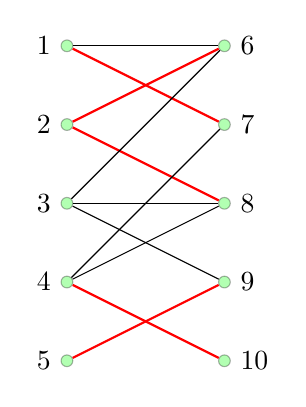
\begin{tikzpicture}
                \node[circle, draw=black, inner sep=1.5pt, fill=green, opacity=0.3, label={180:1}] (1) at (0, 0) {};
                \node[circle, draw=black, inner sep=1.5pt, fill=green, opacity=0.3, label={180:2}] (2) at (0, -1) {};
                \node[circle, draw=black, inner sep=1.5pt, fill=green, opacity=0.3, label={180:3}] (3) at (0, -2) {};
                \node[circle, draw=black, inner sep=1.5pt, fill=green, opacity=0.3, label={180:4}] (4) at (0, -3) {};
                \node[circle, draw=black, inner sep=1.5pt, fill=green, opacity=0.3, label={180:5}] (5) at (0, -4) {};
                \node[circle, draw=black, inner sep=1.5pt, fill=green, opacity=0.3, label={0:6}] (6) at (2, 0) {};
                \node[circle, draw=black, inner sep=1.5pt, fill=green, opacity=0.3, label={0:7}] (7) at (2, -1) {};
                \node[circle, draw=black, inner sep=1.5pt, fill=green, opacity=0.3, label={0:8}] (8) at (2, -2) {};
                \node[circle, draw=black, inner sep=1.5pt, fill=green, opacity=0.3, label={0:9}] (9) at (2, -3) {};
                \node[circle, draw=black, inner sep=1.5pt, fill=green, opacity=0.3, label={0:10}] (10) at (2, -4) {};
            
                \draw (1) -- (6);
                \draw[red, thick] (1) -- (7);
                \draw[red, thick] (2) -- (6);
                \draw[red, thick] (2) -- (8);
                \draw (3) -- (6);
                \draw (3) -- (8);
                \draw (3) -- (9);
                \draw (4) -- (7);
                \draw (4) -- (8);
                \draw[red, thick] (4) -- (10);
                \draw[red, thick] (5) -- (9);
            \end{tikzpicture}
            \caption{Not a matching- vertex 2 has 2 matching edges}
        \end{subfigure}
        \hfill
        \begin{subfigure}{0.45\textwidth}
            \centering
            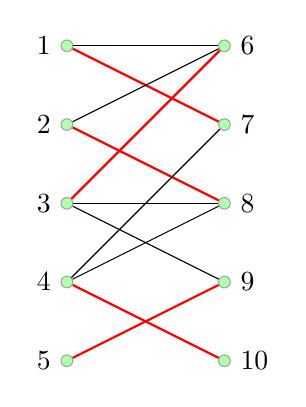
\begin{tikzpicture}
                \node[circle, draw=black, inner sep=1.5pt, fill=green, opacity=0.3, label={180:1}] (1) at (0, 0) {};
                \node[circle, draw=black, inner sep=1.5pt, fill=green, opacity=0.3, label={180:2}] (2) at (0, -1) {};
                \node[circle, draw=black, inner sep=1.5pt, fill=green, opacity=0.3, label={180:3}] (3) at (0, -2) {};
                \node[circle, draw=black, inner sep=1.5pt, fill=green, opacity=0.3, label={180:4}] (4) at (0, -3) {};
                \node[circle, draw=black, inner sep=1.5pt, fill=green, opacity=0.3, label={180:5}] (5) at (0, -4) {};
                \node[circle, draw=black, inner sep=1.5pt, fill=green, opacity=0.3, label={0:6}] (6) at (2, 0) {};
                \node[circle, draw=black, inner sep=1.5pt, fill=green, opacity=0.3, label={0:7}] (7) at (2, -1) {};
                \node[circle, draw=black, inner sep=1.5pt, fill=green, opacity=0.3, label={0:8}] (8) at (2, -2) {};
                \node[circle, draw=black, inner sep=1.5pt, fill=green, opacity=0.3, label={0:9}] (9) at (2, -3) {};
                \node[circle, draw=black, inner sep=1.5pt, fill=green, opacity=0.3, label={0:10}] (10) at (2, -4) {};
            
                \draw (1) -- (6);
                \draw[red, thick] (1) -- (7);
                \draw (2) -- (6);
                \draw[red, thick] (2) -- (8);
                \draw[red, thick] (3) -- (6);
                \draw (3) -- (8);
                \draw (3) -- (9);
                \draw (4) -- (7);
                \draw (4) -- (8);
                \draw[red, thick] (4) -- (10);
                \draw[red, thick] (5) -- (9);
            \end{tikzpicture}
            \caption{A matching}
        \end{subfigure}
    \end{figure}
    \noindent A \emph{maximum cardinality matching} is a matching that has the highest number of edges. A maximum matching is \emph{perfect} if it has cardinality $|V|/2$, i.e. every vertex is part of some edge in the matching. The example above shows a perfect matching. Not every bipartile graph has a perfect matching, such as the graph below:
    \begin{figure}[H]
        \centering
        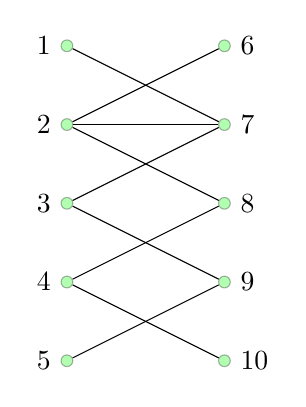
\begin{tikzpicture}
            \node[circle, draw=black, inner sep=1.5pt, fill=green, opacity=0.3, label={180:1}] (1) at (0, 0) {};
            \node[circle, draw=black, inner sep=1.5pt, fill=green, opacity=0.3, label={180:2}] (2) at (0, -1) {};
            \node[circle, draw=black, inner sep=1.5pt, fill=green, opacity=0.3, label={180:3}] (3) at (0, -2) {};
            \node[circle, draw=black, inner sep=1.5pt, fill=green, opacity=0.3, label={180:4}] (4) at (0, -3) {};
            \node[circle, draw=black, inner sep=1.5pt, fill=green, opacity=0.3, label={180:5}] (5) at (0, -4) {};
            \node[circle, draw=black, inner sep=1.5pt, fill=green, opacity=0.3, label={0:6}] (6) at (2, 0) {};
            \node[circle, draw=black, inner sep=1.5pt, fill=green, opacity=0.3, label={0:7}] (7) at (2, -1) {};
            \node[circle, draw=black, inner sep=1.5pt, fill=green, opacity=0.3, label={0:8}] (8) at (2, -2) {};
            \node[circle, draw=black, inner sep=1.5pt, fill=green, opacity=0.3, label={0:9}] (9) at (2, -3) {};
            \node[circle, draw=black, inner sep=1.5pt, fill=green, opacity=0.3, label={0:10}] (10) at (2, -4) {};
        
            \draw (1) -- (7);
            \draw (2) -- (6);
            \draw (2) -- (7);
            \draw (2) -- (8);
            \draw (3) -- (7);
            \draw (3) -- (9);
            \draw (4) -- (8);
            \draw (4) -- (10);
            \draw (5) -- (9);
        \end{tikzpicture}
    \end{figure}
    \noindent We will prove this by a contradiction. So, assume that this graph has a perfect matching. In that case, every vertex with just 1 edge will be part of the matching subset. This means that the red edges given below are part of the matching subset:
    \begin{figure}[H]
        \centering
        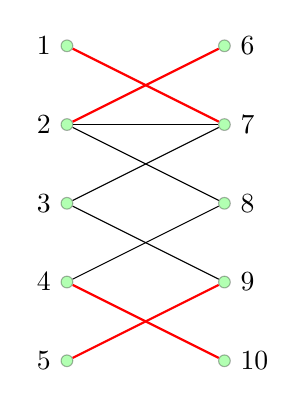
\begin{tikzpicture}
            \node[circle, draw=black, inner sep=1.5pt, fill=green, opacity=0.3, label={180:1}] (1) at (0, 0) {};
            \node[circle, draw=black, inner sep=1.5pt, fill=green, opacity=0.3, label={180:2}] (2) at (0, -1) {};
            \node[circle, draw=black, inner sep=1.5pt, fill=green, opacity=0.3, label={180:3}] (3) at (0, -2) {};
            \node[circle, draw=black, inner sep=1.5pt, fill=green, opacity=0.3, label={180:4}] (4) at (0, -3) {};
            \node[circle, draw=black, inner sep=1.5pt, fill=green, opacity=0.3, label={180:5}] (5) at (0, -4) {};
            \node[circle, draw=black, inner sep=1.5pt, fill=green, opacity=0.3, label={0:6}] (6) at (2, 0) {};
            \node[circle, draw=black, inner sep=1.5pt, fill=green, opacity=0.3, label={0:7}] (7) at (2, -1) {};
            \node[circle, draw=black, inner sep=1.5pt, fill=green, opacity=0.3, label={0:8}] (8) at (2, -2) {};
            \node[circle, draw=black, inner sep=1.5pt, fill=green, opacity=0.3, label={0:9}] (9) at (2, -3) {};
            \node[circle, draw=black, inner sep=1.5pt, fill=green, opacity=0.3, label={0:10}] (10) at (2, -4) {};
        
            \draw[red, thick] (1) -- (7);
            \draw[red, thick] (2) -- (6);
            \draw (2) -- (7);
            \draw (2) -- (8);
            \draw (3) -- (7);
            \draw (3) -- (9);
            \draw (4) -- (8);
            \draw[red, thick] (4) -- (10);
            \draw[red, thick] (5) -- (9);
        \end{tikzpicture}
    \end{figure}
    \noindent Now, since there is a perfect matching, we must be able to add precisely one further edge that will incorporate both the vertices 3 and 8. However, there is no edge between 3 and 8, and adding any other edge would only incorporate one of the vertices (and break the match property). So, this graph does not have a perfect matching. In fact, what we have above is the maximum cardinality matching for the graph.
    
    We will now construct an algorithm to compute the edges that form a maximum cardinality matching. If we did this using brute force, we would need to go through all the permutation of the edges and check whether it is a matching, and if so, whether it is also the maximum (up to that point during the algorithm). This will take $O(m!)$ time, where $m$ is the number of edges in the graph, and is essentially intractable. 

    We shall now look for a better algorithm, which has complexity $O(m^3)$. This uses the concept of finding an \emph{augmenting path} in the current matching to increase, if possible, the size of the matching by 1. The advantage we have in this case is that if we cannot find an augmenting path, then we have found the maximum cardinality matching. At the start, we have an empty matching, from which we increment the size of the matching by 1 until this is not possible, by finding an augmenting path.

    Before defining an augmenting path, we illustrate how this works. So, assume that we are at the following matching:
    \begin{figure}[H]
        \centering
        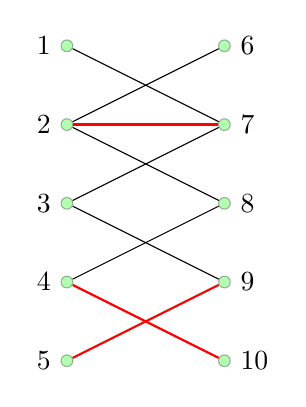
\begin{tikzpicture}
            \node[circle, draw=black, inner sep=1.5pt, fill=green, opacity=0.3, label={180:1}] (1) at (0, 0) {};
            \node[circle, draw=black, inner sep=1.5pt, fill=green, opacity=0.3, label={180:2}] (2) at (0, -1) {};
            \node[circle, draw=black, inner sep=1.5pt, fill=green, opacity=0.3, label={180:3}] (3) at (0, -2) {};
            \node[circle, draw=black, inner sep=1.5pt, fill=green, opacity=0.3, label={180:4}] (4) at (0, -3) {};
            \node[circle, draw=black, inner sep=1.5pt, fill=green, opacity=0.3, label={180:5}] (5) at (0, -4) {};
            \node[circle, draw=black, inner sep=1.5pt, fill=green, opacity=0.3, label={0:6}] (6) at (2, 0) {};
            \node[circle, draw=black, inner sep=1.5pt, fill=green, opacity=0.3, label={0:7}] (7) at (2, -1) {};
            \node[circle, draw=black, inner sep=1.5pt, fill=green, opacity=0.3, label={0:8}] (8) at (2, -2) {};
            \node[circle, draw=black, inner sep=1.5pt, fill=green, opacity=0.3, label={0:9}] (9) at (2, -3) {};
            \node[circle, draw=black, inner sep=1.5pt, fill=green, opacity=0.3, label={0:10}] (10) at (2, -4) {};
        
            \draw (1) -- (7);
            \draw (2) -- (6);
            \draw[red, thick] (2) -- (7);
            \draw (2) -- (8);
            \draw (3) -- (7);
            \draw (3) -- (9);
            \draw (4) -- (8);
            \draw[red, thick] (4) -- (10);
            \draw[red, thick] (5) -- (9);
        \end{tikzpicture}
    \end{figure}
    \noindent We can find an augmenting path here, which is shown below.
    \begin{figure}[H]
        \centering
        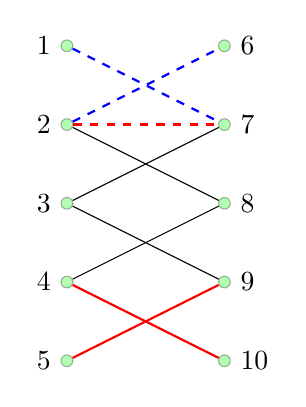
\begin{tikzpicture}
            \node[circle, draw=black, inner sep=1.5pt, fill=green, opacity=0.3, label={180:1}] (1) at (0, 0) {};
            \node[circle, draw=black, inner sep=1.5pt, fill=green, opacity=0.3, label={180:2}] (2) at (0, -1) {};
            \node[circle, draw=black, inner sep=1.5pt, fill=green, opacity=0.3, label={180:3}] (3) at (0, -2) {};
            \node[circle, draw=black, inner sep=1.5pt, fill=green, opacity=0.3, label={180:4}] (4) at (0, -3) {};
            \node[circle, draw=black, inner sep=1.5pt, fill=green, opacity=0.3, label={180:5}] (5) at (0, -4) {};
            \node[circle, draw=black, inner sep=1.5pt, fill=green, opacity=0.3, label={0:6}] (6) at (2, 0) {};
            \node[circle, draw=black, inner sep=1.5pt, fill=green, opacity=0.3, label={0:7}] (7) at (2, -1) {};
            \node[circle, draw=black, inner sep=1.5pt, fill=green, opacity=0.3, label={0:8}] (8) at (2, -2) {};
            \node[circle, draw=black, inner sep=1.5pt, fill=green, opacity=0.3, label={0:9}] (9) at (2, -3) {};
            \node[circle, draw=black, inner sep=1.5pt, fill=green, opacity=0.3, label={0:10}] (10) at (2, -4) {};
        
            \draw[blue, thick, dashed] (1) -- (7);
            \draw[blue, thick, dashed] (2) -- (6);
            \draw[red, dashed, thick] (2) -- (7);
            \draw (2) -- (8);
            \draw (3) -- (7);
            \draw (3) -- (9);
            \draw (4) -- (8);
            \draw[red, thick] (4) -- (10);
            \draw[red, thick] (5) -- (9);
        \end{tikzpicture}
    \end{figure}
    \noindent The augmenting path is the dashed path from the vertex 1 to 6 (or vice versa). An augmenting path alternates between edges in the match and not in the match, and helps us extend the cardinality of the matching. In this case, we remove the edge 2-7 from the matching (the dashed red edge), and replace it with 1-7 and 2-6 (the dashed blue edges). This gives us the following matching:
    \begin{figure}[H]
        \centering
        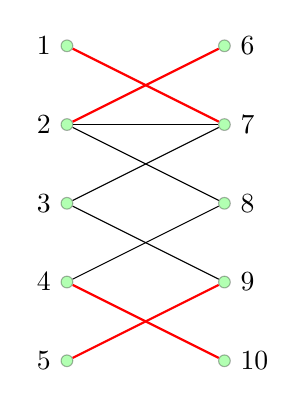
\begin{tikzpicture}
            \node[circle, draw=black, inner sep=1.5pt, fill=green, opacity=0.3, label={180:1}] (1) at (0, 0) {};
            \node[circle, draw=black, inner sep=1.5pt, fill=green, opacity=0.3, label={180:2}] (2) at (0, -1) {};
            \node[circle, draw=black, inner sep=1.5pt, fill=green, opacity=0.3, label={180:3}] (3) at (0, -2) {};
            \node[circle, draw=black, inner sep=1.5pt, fill=green, opacity=0.3, label={180:4}] (4) at (0, -3) {};
            \node[circle, draw=black, inner sep=1.5pt, fill=green, opacity=0.3, label={180:5}] (5) at (0, -4) {};
            \node[circle, draw=black, inner sep=1.5pt, fill=green, opacity=0.3, label={0:6}] (6) at (2, 0) {};
            \node[circle, draw=black, inner sep=1.5pt, fill=green, opacity=0.3, label={0:7}] (7) at (2, -1) {};
            \node[circle, draw=black, inner sep=1.5pt, fill=green, opacity=0.3, label={0:8}] (8) at (2, -2) {};
            \node[circle, draw=black, inner sep=1.5pt, fill=green, opacity=0.3, label={0:9}] (9) at (2, -3) {};
            \node[circle, draw=black, inner sep=1.5pt, fill=green, opacity=0.3, label={0:10}] (10) at (2, -4) {};
        
            \draw[red, thick] (1) -- (7);
            \draw[red, thick] (2) -- (6);
            \draw (2) -- (7);
            \draw (2) -- (8);
            \draw (3) -- (7);
            \draw (3) -- (9);
            \draw (4) -- (8);
            \draw[red, thick] (4) -- (10);
            \draw[red, thick] (5) -- (9);
        \end{tikzpicture}
    \end{figure}
    \noindent As we were able to find an augmenting path, we have been able to extend the matching subset by 1.

    We now build to the definition of augmenting path. In a matching $M$, we say that a vertex $v$ is \emph{matching} if it is part of some edge in the matching subset. If the edge goes from $v$ to $u$, then we say that $u$ and $v$ are \emph{mates}. If the vertex $v$ is not matched, then it is \emph{exposed}. An \emph{alternating path} alternates between edges in $M$ and edges not in $M$. An \emph{augmenting path} is an alternating path that starts and ends at exposed vertices.

    An augmenting path allows us to increase the length of the matching subset- an augmenting path has odd length (if it had even length, then it must end at an exposed vertex), so there is one more non-matching edge in the augmenting path than a matching edge. So, when we replace the matching edges with the non-matching edges, we still have a match (we are swapping the mates for the exposed vertices, and the unexposed vertices originally had no match). Moreover, if there is no augmenting path from any of the unexposed vertices, then we are at a maximum cardinality match.

    We will now consider the algorithm in general.
\begin{lstlisting}[language=pseudocode]
List<Edge> maximumMatching(Graph graph) {
    List<Edge> matching = [];
    Vertex augmentedPath = getAugmentedPath(graph.leftVertices);
    while (augmentedPath != null) {
        matching = augment(augmentedPath);
        augmentedPath = graph.getAugmentedPath();
    }
    return matching;
}
\end{lstlisting}
    The function \texttt{getAugmentedPath} tries to find an augmented path in the bipartile graph given its `left' vertices, and returns the final vertex in the path. The function \texttt{augment} takes an augmented path and selects the right edges to add to the matching.

    Next, we look at the method \texttt{getAugmentedPath} in detail. It is based on breadth-first search, starting from an unexposed vertex until we get to an unexposed vertex `on the same side'. As we saw in the algorithm above, we will only have a look at the left vertices. The following is the algorithm:
\begin{lstlisting}[language=pseudocode]
Vertex getAugmentedPath(List<Vertex> leftVertices) {
    Vertex startVertex = leftVertices.first((v) => v.isUnexposed);
    // no startVertex => every left vertex is exposed 
    if (startVertex == null) {
        return null;
    }

    // Do a DFS to find an unexposed vertex
    Queue<Vertex> queue = Queue(startVertex);
    while (queue.isNotEmpty) {
        Vertex vertex = queue.remove();
        List<Edge> edges = vertex.edges;

        for (int i=0; i<edges.length; i++) {
            Vertex range = edges[i].range;
            if (range.isVisited) {
                range.predecessorEdge = edges[i];
                if (range.isUnexposed) {
                    return range;
                } else {
                    queue.add(range.mate);
                }
            }
        }
    }

    // not possible to find a path between two unexposed vertices
    return null;
}
\end{lstlisting}
    We can then \texttt{augment} to find the matching path as follows:
\begin{lstlisting}[language=pseudocode]
List<Edge> augment(Vertex endVertex) {
    List<Edge> edges = [];
    Vertex vertex = endVertex;
    Edge edge = endVertex.predecessorEdge;

    while (edge != null) {
        Vertex temp = edge.range.mate;
        edge.range.mate = vertex;
        vertex.mate = edge.range;
        edges.add(edge);

        vertex = temp;
        edge = vertex.predecessorEdge;
    }

    return edges;
}
\end{lstlisting}
    Note that the variable \texttt{vertex} at line 12 cannot be null since it is on the left (and the path goes from a left vertex to another left vertex).

    We will now illustrate how the algorithm works with an example. So, assume that we have the following graph.
    \begin{figure}[H]
        \centering
        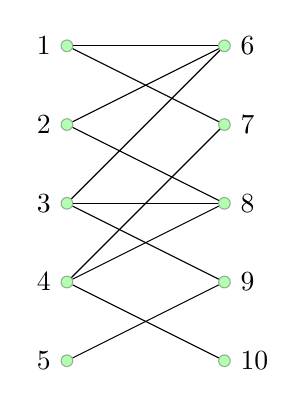
\begin{tikzpicture}
            \node[circle, draw=black, inner sep=1.5pt, fill=green, opacity=0.3, label={180:1}] (1) at (0, 0) {};
            \node[circle, draw=black, inner sep=1.5pt, fill=green, opacity=0.3, label={180:2}] (2) at (0, -1) {};
            \node[circle, draw=black, inner sep=1.5pt, fill=green, opacity=0.3, label={180:3}] (3) at (0, -2) {};
            \node[circle, draw=black, inner sep=1.5pt, fill=green, opacity=0.3, label={180:4}] (4) at (0, -3) {};
            \node[circle, draw=black, inner sep=1.5pt, fill=green, opacity=0.3, label={180:5}] (5) at (0, -4) {};
            \node[circle, draw=black, inner sep=1.5pt, fill=green, opacity=0.3, label={0:6}] (6) at (2, 0) {};
            \node[circle, draw=black, inner sep=1.5pt, fill=green, opacity=0.3, label={0:7}] (7) at (2, -1) {};
            \node[circle, draw=black, inner sep=1.5pt, fill=green, opacity=0.3, label={0:8}] (8) at (2, -2) {};
            \node[circle, draw=black, inner sep=1.5pt, fill=green, opacity=0.3, label={0:9}] (9) at (2, -3) {};
            \node[circle, draw=black, inner sep=1.5pt, fill=green, opacity=0.3, label={0:10}] (10) at (2, -4) {};
        
            \draw (1) -- (6);
            \draw (1) -- (7);
            \draw (2) -- (6);
            \draw (2) -- (8);
            \draw (3) -- (6);
            \draw (3) -- (8);
            \draw (3) -- (9);
            \draw (4) -- (7);
            \draw (4) -- (8);
            \draw (4) -- (10);
            \draw (5) -- (9);
        \end{tikzpicture}
    \end{figure}
    \noindent At the start, we have the empty matching. We will find an augmenting path in the graph.
    \begin{figure}[H]
        \centering
        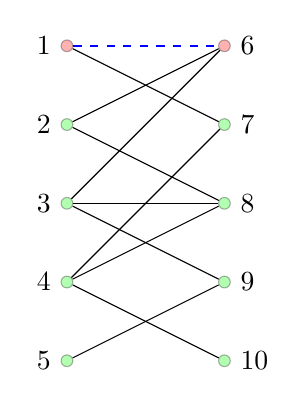
\begin{tikzpicture}
            \node[circle, draw=black, inner sep=1.5pt, fill=red, opacity=0.3, label={180:1}] (1) at (0, 0) {};
            \node[circle, draw=black, inner sep=1.5pt, fill=green, opacity=0.3, label={180:2}] (2) at (0, -1) {};
            \node[circle, draw=black, inner sep=1.5pt, fill=green, opacity=0.3, label={180:3}] (3) at (0, -2) {};
            \node[circle, draw=black, inner sep=1.5pt, fill=green, opacity=0.3, label={180:4}] (4) at (0, -3) {};
            \node[circle, draw=black, inner sep=1.5pt, fill=green, opacity=0.3, label={180:5}] (5) at (0, -4) {};
            \node[circle, draw=black, inner sep=1.5pt, fill=red, opacity=0.3, label={0:6}] (6) at (2, 0) {};
            \node[circle, draw=black, inner sep=1.5pt, fill=green, opacity=0.3, label={0:7}] (7) at (2, -1) {};
            \node[circle, draw=black, inner sep=1.5pt, fill=green, opacity=0.3, label={0:8}] (8) at (2, -2) {};
            \node[circle, draw=black, inner sep=1.5pt, fill=green, opacity=0.3, label={0:9}] (9) at (2, -3) {};
            \node[circle, draw=black, inner sep=1.5pt, fill=green, opacity=0.3, label={0:10}] (10) at (2, -4) {};
        
            \draw[blue, dashed, thick] (1) -- (6);
            \draw (1) -- (7);
            \draw (2) -- (6);
            \draw (2) -- (8);
            \draw (3) -- (6);
            \draw (3) -- (8);
            \draw (3) -- (9);
            \draw (4) -- (7);
            \draw (4) -- (8);
            \draw (4) -- (10);
            \draw (5) -- (9);
        \end{tikzpicture}
    \end{figure}
    \noindent We denote by red a visited vertex during this iteration. The first unexposed vertex we find is vertex 1, which has an edge to vertex 6. So, we add this edge to the matching. This gives us the following matching.
    \begin{figure}[H]
        \centering
        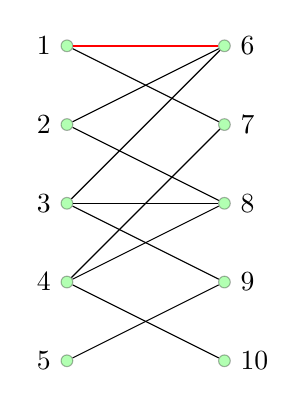
\begin{tikzpicture}
            \node[circle, draw=black, inner sep=1.5pt, fill=green, opacity=0.3, label={180:1}] (1) at (0, 0) {};
            \node[circle, draw=black, inner sep=1.5pt, fill=green, opacity=0.3, label={180:2}] (2) at (0, -1) {};
            \node[circle, draw=black, inner sep=1.5pt, fill=green, opacity=0.3, label={180:3}] (3) at (0, -2) {};
            \node[circle, draw=black, inner sep=1.5pt, fill=green, opacity=0.3, label={180:4}] (4) at (0, -3) {};
            \node[circle, draw=black, inner sep=1.5pt, fill=green, opacity=0.3, label={180:5}] (5) at (0, -4) {};
            \node[circle, draw=black, inner sep=1.5pt, fill=green, opacity=0.3, label={0:6}] (6) at (2, 0) {};
            \node[circle, draw=black, inner sep=1.5pt, fill=green, opacity=0.3, label={0:7}] (7) at (2, -1) {};
            \node[circle, draw=black, inner sep=1.5pt, fill=green, opacity=0.3, label={0:8}] (8) at (2, -2) {};
            \node[circle, draw=black, inner sep=1.5pt, fill=green, opacity=0.3, label={0:9}] (9) at (2, -3) {};
            \node[circle, draw=black, inner sep=1.5pt, fill=green, opacity=0.3, label={0:10}] (10) at (2, -4) {};
        
            \draw[red, thick] (1) -- (6);
            \draw (1) -- (7);
            \draw (2) -- (6);
            \draw (2) -- (8);
            \draw (3) -- (6);
            \draw (3) -- (8);
            \draw (3) -- (9);
            \draw (4) -- (7);
            \draw (4) -- (8);
            \draw (4) -- (10);
            \draw (5) -- (9);
        \end{tikzpicture}
    \end{figure}
    \noindent We will now search for another augmenting path.
    \begin{figure}[H]
        \centering
        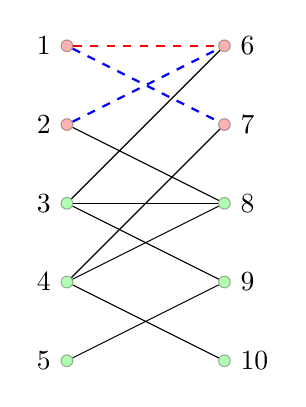
\begin{tikzpicture}
            \node[circle, draw=black, inner sep=1.5pt, fill=red, opacity=0.3, label={180:1}] (1) at (0, 0) {};
            \node[circle, draw=black, inner sep=1.5pt, fill=red, opacity=0.3, label={180:2}] (2) at (0, -1) {};
            \node[circle, draw=black, inner sep=1.5pt, fill=green, opacity=0.3, label={180:3}] (3) at (0, -2) {};
            \node[circle, draw=black, inner sep=1.5pt, fill=green, opacity=0.3, label={180:4}] (4) at (0, -3) {};
            \node[circle, draw=black, inner sep=1.5pt, fill=green, opacity=0.3, label={180:5}] (5) at (0, -4) {};
            \node[circle, draw=black, inner sep=1.5pt, fill=red, opacity=0.3, label={0:6}] (6) at (2, 0) {};
            \node[circle, draw=black, inner sep=1.5pt, fill=red, opacity=0.3, label={0:7}] (7) at (2, -1) {};
            \node[circle, draw=black, inner sep=1.5pt, fill=green, opacity=0.3, label={0:8}] (8) at (2, -2) {};
            \node[circle, draw=black, inner sep=1.5pt, fill=green, opacity=0.3, label={0:9}] (9) at (2, -3) {};
            \node[circle, draw=black, inner sep=1.5pt, fill=green, opacity=0.3, label={0:10}] (10) at (2, -4) {};
        
            \draw[red, dashed, thick] (1) -- (6);
            \draw[blue, dashed, thick] (1) -- (7);
            \draw[blue, dashed, thick] (2) -- (6);
            \draw (2) -- (8);
            \draw (3) -- (6);
            \draw (3) -- (8);
            \draw (3) -- (9);
            \draw (4) -- (7);
            \draw (4) -- (8);
            \draw (4) -- (10);
            \draw (5) -- (9);
        \end{tikzpicture}
    \end{figure}
    \noindent In this case, the augmenting path starts at vertex 2. We first find its edge to vertex 6. This is an exposed vertex, so we add its mate vertex 1 to the queue. From vertex 1, we cannot take the edge to vertex 6 since it has already been visited, so we take the edge to vertex 7. This vertex is exposed, so the augmenting path is complete. Using this, we get the following matching:
    \begin{figure}[H]
        \centering
        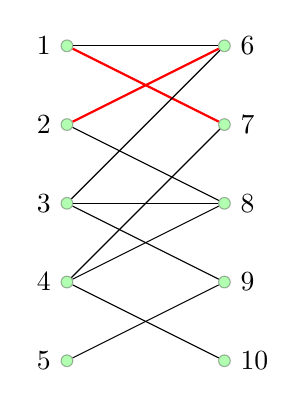
\begin{tikzpicture}
            \node[circle, draw=black, inner sep=1.5pt, fill=green, opacity=0.3, label={180:1}] (1) at (0, 0) {};
            \node[circle, draw=black, inner sep=1.5pt, fill=green, opacity=0.3, label={180:2}] (2) at (0, -1) {};
            \node[circle, draw=black, inner sep=1.5pt, fill=green, opacity=0.3, label={180:3}] (3) at (0, -2) {};
            \node[circle, draw=black, inner sep=1.5pt, fill=green, opacity=0.3, label={180:4}] (4) at (0, -3) {};
            \node[circle, draw=black, inner sep=1.5pt, fill=green, opacity=0.3, label={180:5}] (5) at (0, -4) {};
            \node[circle, draw=black, inner sep=1.5pt, fill=green, opacity=0.3, label={0:6}] (6) at (2, 0) {};
            \node[circle, draw=black, inner sep=1.5pt, fill=green, opacity=0.3, label={0:7}] (7) at (2, -1) {};
            \node[circle, draw=black, inner sep=1.5pt, fill=green, opacity=0.3, label={0:8}] (8) at (2, -2) {};
            \node[circle, draw=black, inner sep=1.5pt, fill=green, opacity=0.3, label={0:9}] (9) at (2, -3) {};
            \node[circle, draw=black, inner sep=1.5pt, fill=green, opacity=0.3, label={0:10}] (10) at (2, -4) {};
        
            \draw (1) -- (6);
            \draw[red, thick] (1) -- (7);
            \draw[red, thick] (2) -- (6);
            \draw (2) -- (8);
            \draw (3) -- (6);
            \draw (3) -- (8);
            \draw (3) -- (9);
            \draw (4) -- (7);
            \draw (4) -- (8);
            \draw (4) -- (10);
            \draw (5) -- (9);
        \end{tikzpicture}
    \end{figure}
    \noindent We can continue using the augmenting algorithm to get to the following matching:
    \begin{figure}[H]
        \centering
        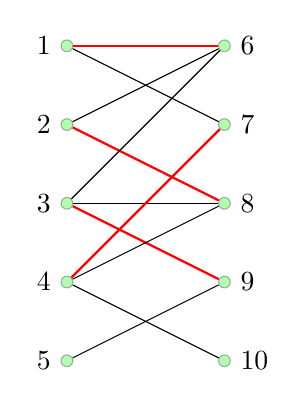
\begin{tikzpicture}
            \node[circle, draw=black, inner sep=1.5pt, fill=green, opacity=0.3, label={180:1}] (1) at (0, 0) {};
            \node[circle, draw=black, inner sep=1.5pt, fill=green, opacity=0.3, label={180:2}] (2) at (0, -1) {};
            \node[circle, draw=black, inner sep=1.5pt, fill=green, opacity=0.3, label={180:3}] (3) at (0, -2) {};
            \node[circle, draw=black, inner sep=1.5pt, fill=green, opacity=0.3, label={180:4}] (4) at (0, -3) {};
            \node[circle, draw=black, inner sep=1.5pt, fill=green, opacity=0.3, label={180:5}] (5) at (0, -4) {};
            \node[circle, draw=black, inner sep=1.5pt, fill=green, opacity=0.3, label={0:6}] (6) at (2, 0) {};
            \node[circle, draw=black, inner sep=1.5pt, fill=green, opacity=0.3, label={0:7}] (7) at (2, -1) {};
            \node[circle, draw=black, inner sep=1.5pt, fill=green, opacity=0.3, label={0:8}] (8) at (2, -2) {};
            \node[circle, draw=black, inner sep=1.5pt, fill=green, opacity=0.3, label={0:9}] (9) at (2, -3) {};
            \node[circle, draw=black, inner sep=1.5pt, fill=green, opacity=0.3, label={0:10}] (10) at (2, -4) {};
        
            \draw[red, thick] (1) -- (6);
            \draw (1) -- (7);
            \draw (2) -- (6);
            \draw[red, thick] (2) -- (8);
            \draw (3) -- (6);
            \draw (3) -- (8);
            \draw[red, thick] (3) -- (9);
            \draw[red, thick] (4) -- (7);
            \draw (4) -- (8);
            \draw (4) -- (10);
            \draw (5) -- (9);
        \end{tikzpicture}
    \end{figure}    
    \noindent Now, we will try finding another augmenting path.
    \begin{figure}[H]
        \centering
        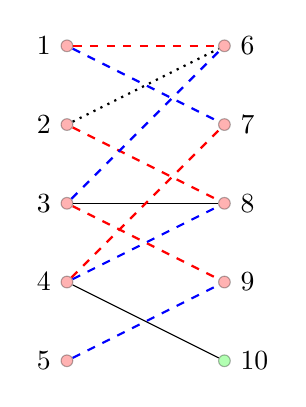
\begin{tikzpicture}
            \node[circle, draw=black, inner sep=1.5pt, fill=red, opacity=0.3, label={180:1}] (1) at (0, 0) {};
            \node[circle, draw=black, inner sep=1.5pt, fill=red, opacity=0.3, label={180:2}] (2) at (0, -1) {};
            \node[circle, draw=black, inner sep=1.5pt, fill=red, opacity=0.3, label={180:3}] (3) at (0, -2) {};
            \node[circle, draw=black, inner sep=1.5pt, fill=red, opacity=0.3, label={180:4}] (4) at (0, -3) {};
            \node[circle, draw=black, inner sep=1.5pt, fill=red, opacity=0.3, label={180:5}] (5) at (0, -4) {};
            \node[circle, draw=black, inner sep=1.5pt, fill=red, opacity=0.3, label={0:6}] (6) at (2, 0) {};
            \node[circle, draw=black, inner sep=1.5pt, fill=red, opacity=0.3, label={0:7}] (7) at (2, -1) {};
            \node[circle, draw=black, inner sep=1.5pt, fill=red, opacity=0.3, label={0:8}] (8) at (2, -2) {};
            \node[circle, draw=black, inner sep=1.5pt, fill=red, opacity=0.3, label={0:9}] (9) at (2, -3) {};
            \node[circle, draw=black, inner sep=1.5pt, fill=green, opacity=0.3, label={0:10}] (10) at (2, -4) {};
        
            \draw[red, dashed, thick] (1) -- (6);
            \draw[blue, dashed, thick] (1) -- (7);
            \draw[dotted, thick] (2) -- (6);
            \draw[red, dashed, thick] (2) -- (8);
            \draw[blue, thick, dashed] (3) -- (6);
            \draw (3) -- (8);
            \draw[red, dashed, thick] (3) -- (9);
            \draw[red, dashed, thick] (4) -- (7);
            \draw[blue, dashed, thick] (4) -- (8);
            \draw (4) -- (10);
            \draw[blue, thick, dashed] (5) -- (9);
        \end{tikzpicture}
    \end{figure}
    \noindent We start with the unexposed vertex 5, and take its edge to vertex 9. This is exposed, so we add its mate to the queue. This process continues as expected, until we add vertex 4 to the queue. We first take the edge it has to vertex 8, at which point we add vertex 3 to the queue. However, every edge that vertex 2 has goes to a visited vertex. So, we have to backtrack- we take the other edge from vertex 4.
    \begin{figure}[H]
        \centering
        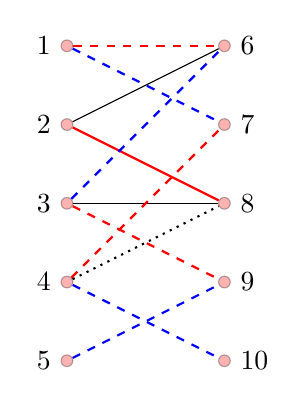
\begin{tikzpicture}
            \node[circle, draw=black, inner sep=1.5pt, fill=red, opacity=0.3, label={180:1}] (1) at (0, 0) {};
            \node[circle, draw=black, inner sep=1.5pt, fill=red, opacity=0.3, label={180:2}] (2) at (0, -1) {};
            \node[circle, draw=black, inner sep=1.5pt, fill=red, opacity=0.3, label={180:3}] (3) at (0, -2) {};
            \node[circle, draw=black, inner sep=1.5pt, fill=red, opacity=0.3, label={180:4}] (4) at (0, -3) {};
            \node[circle, draw=black, inner sep=1.5pt, fill=red, opacity=0.3, label={180:5}] (5) at (0, -4) {};
            \node[circle, draw=black, inner sep=1.5pt, fill=red, opacity=0.3, label={0:6}] (6) at (2, 0) {};
            \node[circle, draw=black, inner sep=1.5pt, fill=red, opacity=0.3, label={0:7}] (7) at (2, -1) {};
            \node[circle, draw=black, inner sep=1.5pt, fill=red, opacity=0.3, label={0:8}] (8) at (2, -2) {};
            \node[circle, draw=black, inner sep=1.5pt, fill=red, opacity=0.3, label={0:9}] (9) at (2, -3) {};
            \node[circle, draw=black, inner sep=1.5pt, fill=red, opacity=0.3, label={0:10}] (10) at (2, -4) {};
        
            \draw[red, dashed, thick] (1) -- (6);
            \draw[blue, dashed, thick] (1) -- (7);
            \draw (2) -- (6);
            \draw[red, thick] (2) -- (8);
            \draw[blue, thick, dashed] (3) -- (6);
            \draw (3) -- (8);
            \draw[red, dashed, thick] (3) -- (9);
            \draw[red, dashed, thick] (4) -- (7);
            \draw[thick, dotted] (4) -- (8);
            \draw[blue, dashed, thick] (4) -- (10);
            \draw[blue, thick, dashed] (5) -- (9);
        \end{tikzpicture}
    \end{figure}
    \noindent In this case, we take the edge from vertex 4 to vertex 10. This is an exposed vertex, so we have found the augmenting path. Moreover, there is no unexposed (left) vertex, so the algorithm terminates with the following matching:
    \begin{figure}[H]
        \centering
        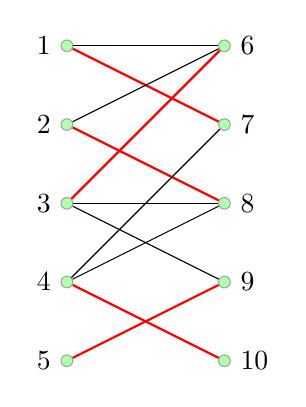
\begin{tikzpicture}
            \node[circle, draw=black, inner sep=1.5pt, fill=green, opacity=0.3, label={180:1}] (1) at (0, 0) {};
            \node[circle, draw=black, inner sep=1.5pt, fill=green, opacity=0.3, label={180:2}] (2) at (0, -1) {};
            \node[circle, draw=black, inner sep=1.5pt, fill=green, opacity=0.3, label={180:3}] (3) at (0, -2) {};
            \node[circle, draw=black, inner sep=1.5pt, fill=green, opacity=0.3, label={180:4}] (4) at (0, -3) {};
            \node[circle, draw=black, inner sep=1.5pt, fill=green, opacity=0.3, label={180:5}] (5) at (0, -4) {};
            \node[circle, draw=black, inner sep=1.5pt, fill=green, opacity=0.3, label={0:6}] (6) at (2, 0) {};
            \node[circle, draw=black, inner sep=1.5pt, fill=green, opacity=0.3, label={0:7}] (7) at (2, -1) {};
            \node[circle, draw=black, inner sep=1.5pt, fill=green, opacity=0.3, label={0:8}] (8) at (2, -2) {};
            \node[circle, draw=black, inner sep=1.5pt, fill=green, opacity=0.3, label={0:9}] (9) at (2, -3) {};
            \node[circle, draw=black, inner sep=1.5pt, fill=green, opacity=0.3, label={0:10}] (10) at (2, -4) {};
        
            \draw (1) -- (6);
            \draw[red, thick] (1) -- (7);
            \draw (2) -- (6);
            \draw[red, thick] (2) -- (8);
            \draw[red, thick] (3) -- (6);
            \draw (3) -- (8);
            \draw (3) -- (9);
            \draw (4) -- (7);
            \draw (4) -- (8);
            \draw[red, thick] (4) -- (10);
            \draw[red, thick] (5) -- (9);
        \end{tikzpicture}
    \end{figure}

    We will now consider the complexity of the algorithm. Assume that $p$ and $q$ are the number of vertices in the two partitions of the graph, and let $|V| = n$ and $|E| = m$. We assume that $p < q$, with $p$ the number of left vertices without loss of generality. The function \texttt{getAugmentedPath} is a version of depth-first search where every second vertex is a left vertex, so it has $O(p + m)$ complexity. The augmenting process has $O(m)$ complexity since we encounter an edge at most once during the iteration. The main loop can run at most $p$ times- during each iteration, we must expose a left vertex. So, the entire algorithm takes $O(p(p+m))$ time. We have $p \leq n$, so this is $O(n(n+m))$. If we further assume that $m = O(n^2)$, we find that the algorithm is $O(n^3)$. The fastest algorithm that is known has complexity $O(\sqrt{n}(n+m))$, and this complexity can also be achieved for non-bipartile graphs.
    \newpage

    \section{Network Flow}
    In this section, we will look at a network (which is a special kind of directed graph), which has a (maximum) capacity along with a flow (a weighted graph) that obeys some rules. We will consider how to compute the maximum flow for a given network.

    A \emph{network} is a directed graph $G = (V, E)$ such that there is a \emph{source} vertex (which has no incoming edge) and a \emph{sink} (which has no outgoing edge), and every edge $(u, v) \in E$ has a non-negative \emph{capacity}, denoted by $c(u, v) \in \mathbb{R}$. For two vertices $u$ and $v$ without any edge between them, we can define their capacity $c(u, v) = 0$. A \emph{flow} in a network $G$ is a function $f \colon E \to \mathbb{R}$ such that it obeys the following:
    \begin{itemize}
        \item capacity constraint: for every edge $(u, v) \in E$, $0 \leq f(u, v) \leq c(u, v)$, i.e. the flow doesn't exceed the capacity; and
        \item flow conservation constraint: for every vertex $v$ that is not the source or the sink, the total incoming flow equals the total outgoing flow.
    \end{itemize}
    The \emph{value} of a flow $f$, denoted by $f$, is the total outgoing flow from the source $s$ (or the total incoming flow to the sink $t$).

    The following example gives a network, with the values denoting the capacity of each edge.
    \begin{figure}[H]
        \centering
        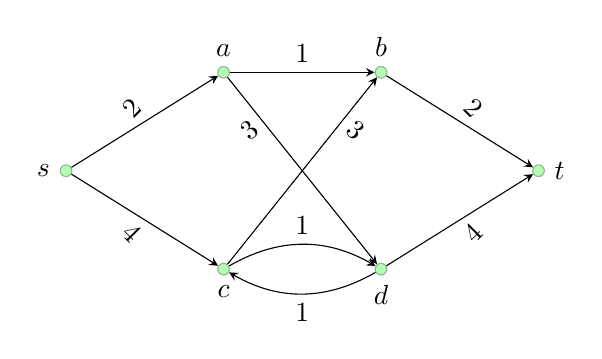
\begin{tikzpicture}
            \node[circle, draw, inner sep=1.5pt, fill=green, opacity=0.3, label={-180:$s$}] (s) at (0, 0) {};
            \node[circle, draw, inner sep=1.5pt, fill=green, opacity=0.3, label={90:$a$}] (a) at (2, 1.25) {};
            \node[circle, draw, inner sep=1.5pt, fill=green, opacity=0.3, label={90:$b$}] (b) at (4, 1.25) {};
            \node[circle, draw, inner sep=1.5pt, fill=green, opacity=0.3, label={-90:$c$}] (c) at (2, -1.25) {};
            \node[circle, draw, inner sep=1.5pt, fill=green, opacity=0.3, label={-90:$d$}] (d) at (4, -1.25) {};
            \node[circle, draw, inner sep=1.5pt, fill=green, opacity=0.3, label={0:$t$}] (t) at (6, 0) {};

            \draw[-stealth] (s) -- node[above, rotate=45] {2} (a);
            \draw[-stealth] (s) -- node[below, rotate=-45] {4} (c);
            \draw[-stealth] (a) -- node[above] {1} (b);
            \draw[-stealth] (b) -- node[above, rotate=-45] {2} (t);
            \draw[-stealth] (d) -- node[below, rotate=45] {4} (t);
            \draw[-stealth] (a) -- node[below left, rotate=40, pos=0.15] {3} (d);
            \draw[-stealth] (c) -- node[below right, rotate=-40, pos=0.85] {3} (b);
            \draw[-stealth] (c) edge[bend left] node[above] {1} (d);
            \draw[-stealth] (d) edge[bend left] node[below] {1} (c);
        \end{tikzpicture}
    \end{figure}
    \noindent A possible flow through the network is the following:
    \begin{figure}[H]
        \centering
        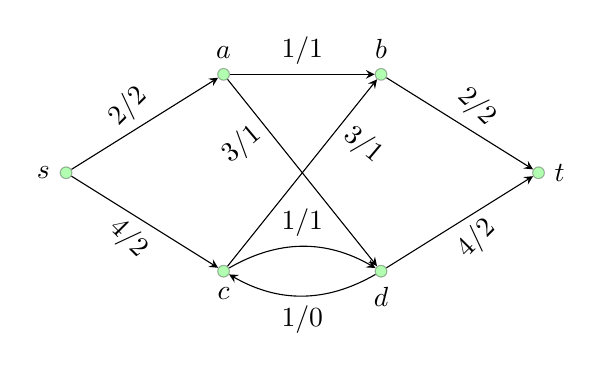
\begin{tikzpicture}
            \node[circle, draw, inner sep=1.5pt, fill=green, opacity=0.3, label={-180:$s$}] (s) at (0, 0) {};
            \node[circle, draw, inner sep=1.5pt, fill=green, opacity=0.3, label={90:$a$}] (a) at (2, 1.25) {};
            \node[circle, draw, inner sep=1.5pt, fill=green, opacity=0.3, label={90:$b$}] (b) at (4, 1.25) {};
            \node[circle, draw, inner sep=1.5pt, fill=green, opacity=0.3, label={-90:$c$}] (c) at (2, -1.25) {};
            \node[circle, draw, inner sep=1.5pt, fill=green, opacity=0.3, label={-90:$d$}] (d) at (4, -1.25) {};
            \node[circle, draw, inner sep=1.5pt, fill=green, opacity=0.3, label={0:$t$}] (t) at (6, 0) {};

            \draw[-stealth] (s) -- node[above, rotate=45] {2/2} (a);
            \draw[-stealth] (s) -- node[below, rotate=-45] {4/2} (c);
            \draw[-stealth] (a) -- node[above] {1/1} (b);
            \draw[-stealth] (b) -- node[above, rotate=-45] {2/2} (t);
            \draw[-stealth] (d) -- node[below, rotate=45] {4/2} (t);
            \draw[-stealth] (a) -- node[below left, rotate=40, pos=0.15] {3/1} (d);
            \draw[-stealth] (c) -- node[below right, rotate=-40, pos=0.85] {3/1} (b);
            \draw[-stealth] (c) edge[bend left] node[above] {1/1} (d);
            \draw[-stealth] (d) edge[bend left] node[below] {1/0} (c);
        \end{tikzpicture}
    \end{figure}
    \noindent We denote an edge by $a/b$, where $a$ is the capacity and $b$ is the flow. We can see that the flow is always non-negative and smaller than the capacity. Moreover, for $a$, $b$, $c$ and $d$, the total incoming flow equals the total outgoing flow, e.g. $s-a$ is the only incoming edge to $a$, with flow $2$, and the two outgoing edges $a - b$ and $a - d$ have total flow $2$. The value of the flow above is 4. We can actually find another flow of higher value. Consider the flow given below:
    \begin{figure}[H]
        \centering
        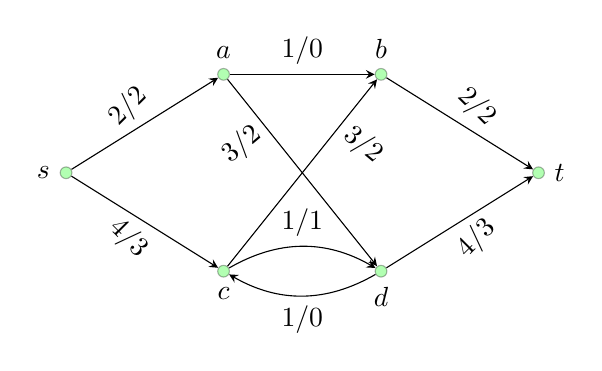
\begin{tikzpicture}
            \node[circle, draw, inner sep=1.5pt, fill=green, opacity=0.3, label={-180:$s$}] (s) at (0, 0) {};
            \node[circle, draw, inner sep=1.5pt, fill=green, opacity=0.3, label={90:$a$}] (a) at (2, 1.25) {};
            \node[circle, draw, inner sep=1.5pt, fill=green, opacity=0.3, label={90:$b$}] (b) at (4, 1.25) {};
            \node[circle, draw, inner sep=1.5pt, fill=green, opacity=0.3, label={-90:$c$}] (c) at (2, -1.25) {};
            \node[circle, draw, inner sep=1.5pt, fill=green, opacity=0.3, label={-90:$d$}] (d) at (4, -1.25) {};
            \node[circle, draw, inner sep=1.5pt, fill=green, opacity=0.3, label={0:$t$}] (t) at (6, 0) {};

            \draw[-stealth] (s) -- node[above, rotate=45] {2/2} (a);
            \draw[-stealth] (s) -- node[below, rotate=-45] {4/3} (c);
            \draw[-stealth] (a) -- node[above] {1/0} (b);
            \draw[-stealth] (b) -- node[above, rotate=-45] {2/2} (t);
            \draw[-stealth] (d) -- node[below, rotate=45] {4/3} (t);
            \draw[-stealth] (a) -- node[below left, rotate=40, pos=0.15] {3/2} (d);
            \draw[-stealth] (c) -- node[below right, rotate=-40, pos=0.85] {3/2} (b);
            \draw[-stealth] (c) edge[bend left] node[above] {1/1} (d);
            \draw[-stealth] (d) edge[bend left] node[below] {1/0} (c);
        \end{tikzpicture}
    \end{figure}
    \noindent We can verify by inspection that we have a flow above. Moreover, it has value 5.
    
    We claim that there is no flow of higher value. Assume, for a contradiction, that there is a flow of value 6. We try to construct such a flow:
    \begin{figure}[H]
        \centering
        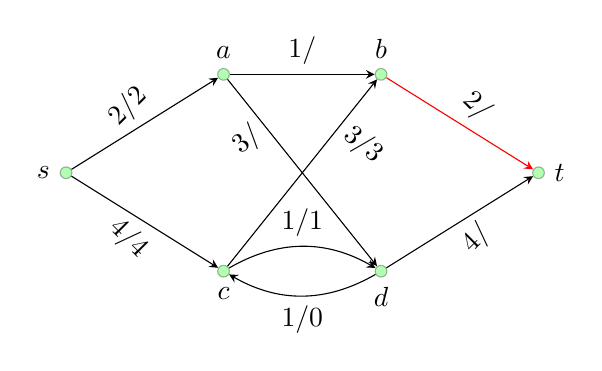
\begin{tikzpicture}
            \node[circle, draw, inner sep=1.5pt, fill=green, opacity=0.3, label={-180:$s$}] (s) at (0, 0) {};
            \node[circle, draw, inner sep=1.5pt, fill=green, opacity=0.3, label={90:$a$}] (a) at (2, 1.25) {};
            \node[circle, draw, inner sep=1.5pt, fill=green, opacity=0.3, label={90:$b$}] (b) at (4, 1.25) {};
            \node[circle, draw, inner sep=1.5pt, fill=green, opacity=0.3, label={-90:$c$}] (c) at (2, -1.25) {};
            \node[circle, draw, inner sep=1.5pt, fill=green, opacity=0.3, label={-90:$d$}] (d) at (4, -1.25) {};
            \node[circle, draw, inner sep=1.5pt, fill=green, opacity=0.3, label={0:$t$}] (t) at (6, 0) {};

            \draw[-stealth] (s) -- node[above, rotate=45] {2/2} (a);
            \draw[-stealth] (s) -- node[below, rotate=-45] {4/4} (c);
            \draw[-stealth] (a) -- node[above] {1/} (b);
            \draw[-stealth, red] (b) -- node[black, above, rotate=-45] {2/} (t);
            \draw[-stealth] (d) -- node[below, rotate=45] {4/} (t);
            \draw[-stealth] (a) -- node[below left, rotate=40, pos=0.15] {3/} (d);
            \draw[-stealth] (c) -- node[below right, rotate=-40, pos=0.85] {3/3} (b);
            \draw[-stealth] (c) edge[bend left] node[above] {1/1} (d);
            \draw[-stealth] (d) edge[bend left] node[below] {1/0} (c);
        \end{tikzpicture}
    \end{figure}
    \noindent Since the sources have total outgoing capacity 6, the outgoing edges from $s$ must be \emph{saturated} (capacity equals flow). This means that $c$ has incoming flow of at least 4. Since the outgoing edges have total capacity 4, the edge $c - d$ has flow 0. Also, the outgoing edges from $c$ must be saturated. In particular, $b$ has incoming flow of at least 3. However, $b$ only has one outgoing edge (given in red), with capacity 2. This is a contradiction- we cannot have a flow of value 6. So, the flow we had above of value 5 is the maximum flow.

    We will now look at an algorithm to find a maximum flow for a network. To do so, we will need to use \emph{augmenting paths}, like in the maximum cardinality matching algorithm. An augmenting path is a path from the source $s$ to the sink $t$ that has edges in $G$, but not necessarily in the direction that it exists in $G$. In particular, an edge $(u, v)$ in the path satisfies one of the following:
    \begin{itemize}
        \item $(u, v)$ is an edge in $G$, and the flow is not equal to the capacity (this is a \emph{forwards-edge})- the difference is called the \emph{slack}, which is greater than 0; or
        \item $(v, u)$ is an edge in $G$, and the flow is non-zero (this is a \emph{backwards-edge}).
    \end{itemize}
    Using an augmented path, we can increase the value of the flow- we increase the flow in the forwards-edges (while ensuring it doesn't cross the capacity) and decrease the flow in backwards-edges (while ensuring it doesn't go below 0). The following is an augmenting path for the network we had above:    
    \begin{figure}[H]
        \centering
        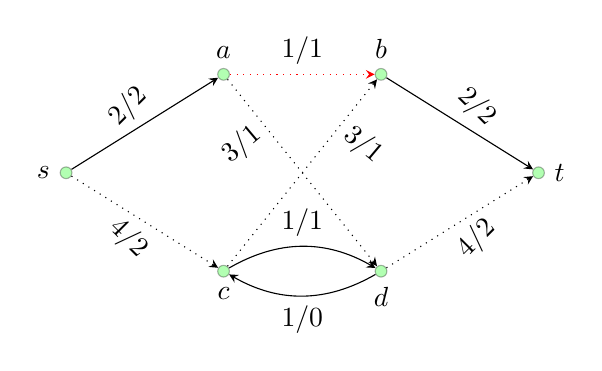
\begin{tikzpicture}
            \node[circle, draw, inner sep=1.5pt, fill=green, opacity=0.3, label={-180:$s$}] (s) at (0, 0) {};
            \node[circle, draw, inner sep=1.5pt, fill=green, opacity=0.3, label={90:$a$}] (a) at (2, 1.25) {};
            \node[circle, draw, inner sep=1.5pt, fill=green, opacity=0.3, label={90:$b$}] (b) at (4, 1.25) {};
            \node[circle, draw, inner sep=1.5pt, fill=green, opacity=0.3, label={-90:$c$}] (c) at (2, -1.25) {};
            \node[circle, draw, inner sep=1.5pt, fill=green, opacity=0.3, label={-90:$d$}] (d) at (4, -1.25) {};
            \node[circle, draw, inner sep=1.5pt, fill=green, opacity=0.3, label={0:$t$}] (t) at (6, 0) {};

            \draw[-stealth] (s) -- node[above, rotate=45] {2/2} (a);
            \draw[-stealth, dotted] (s) -- node[below, rotate=-45] {4/2} (c);
            \draw[-stealth, red, dotted] (a) -- node[above, black] {1/1} (b);
            \draw[-stealth] (b) -- node[above, rotate=-45] {2/2} (t);
            \draw[-stealth, dotted] (d) -- node[below, rotate=45] {4/2} (t);
            \draw[-stealth, dotted] (a) -- node[below left, rotate=40, pos=0.15] {3/1} (d);
            \draw[-stealth, dotted] (c) -- node[below right, rotate=-40, pos=0.85] {3/1} (b);
            \draw[-stealth] (c) edge[bend left] node[above] {1/1} (d);
            \draw[-stealth] (d) edge[bend left] node[below] {1/0} (c);
        \end{tikzpicture}
    \end{figure}
    \noindent The network has flow 4. The augmenting path has 5 edges: $(s, c)$, $(c, b)$, $(b, a)$, $(a, d)$ and $(d, t)$. Only the edge $(b, a)$ is backwards (and given in red). The edge $(s, c)$ has slack 2; the edge $(c, d)$ has slack 2; the flow in the edge $(b, a)$ can be decreased by 1, and so on. We compute the minimum value $m$ corresponding to an edge and change the flow accordingly- we increment the flow by $m$ to a forwards-edge and decrement by $m$ to a backwards-edge. This gives us the following network flow:
    \begin{figure}[H]
        \centering
        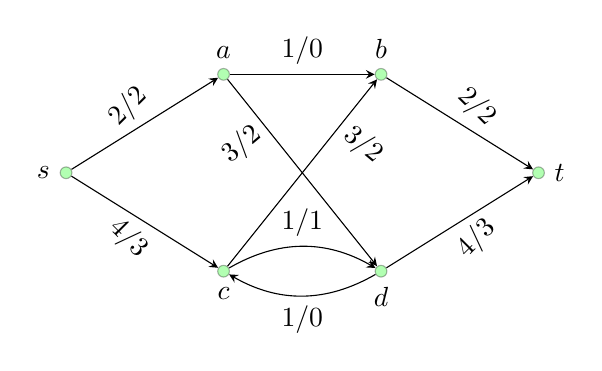
\begin{tikzpicture}
            \node[circle, draw, inner sep=1.5pt, fill=green, opacity=0.3, label={-180:$s$}] (s) at (0, 0) {};
            \node[circle, draw, inner sep=1.5pt, fill=green, opacity=0.3, label={90:$a$}] (a) at (2, 1.25) {};
            \node[circle, draw, inner sep=1.5pt, fill=green, opacity=0.3, label={90:$b$}] (b) at (4, 1.25) {};
            \node[circle, draw, inner sep=1.5pt, fill=green, opacity=0.3, label={-90:$c$}] (c) at (2, -1.25) {};
            \node[circle, draw, inner sep=1.5pt, fill=green, opacity=0.3, label={-90:$d$}] (d) at (4, -1.25) {};
            \node[circle, draw, inner sep=1.5pt, fill=green, opacity=0.3, label={0:$t$}] (t) at (6, 0) {};

            \draw[-stealth] (s) -- node[above, rotate=45] {2/2} (a);
            \draw[-stealth] (s) -- node[below, rotate=-45] {4/3} (c);
            \draw[-stealth] (a) -- node[above] {1/0} (b);
            \draw[-stealth] (b) -- node[above, rotate=-45] {2/2} (t);
            \draw[-stealth] (d) -- node[below, rotate=45] {4/3} (t);
            \draw[-stealth] (a) -- node[below left, rotate=40, pos=0.15] {3/2} (d);
            \draw[-stealth] (c) -- node[below right, rotate=-40, pos=0.85] {3/2} (b);
            \draw[-stealth] (c) edge[bend left] node[above] {1/1} (d);
            \draw[-stealth] (d) edge[bend left] node[below] {1/0} (c);
        \end{tikzpicture}
    \end{figure}
    \noindent This flow has value 5. Every edge leaving the source has to be a forwards-edge (if there was a backwards-edge, then there would be an incoming edge to the source, which is not possible). Hence, the value of the flow must always increase when we augment the flow using the augmenting path.

    Like in the case of the maximum cardinality matching algorithm, a flow is maximum if and only if it has no augmenting path. We saw above that if the flow has an augmenting path, then it is not maximum- we can change the flow by the minimum of the slack/flow so that the value of the flow increases.

    In particular, let $m$ be the minimum of the slacks for forwards edges and flow for backwards edges. We have a new function $f' \colon E \to \mathbb{R}$, based on the previous flow function $f \colon E \to \mathbb{R}$. We will now show $f'$ is actually a flow, i.e. it obeys the capacity and the flow-conservation constraint. First, we consider the capacity constraint:
    \begin{itemize}
        \item the flow we generate will keep the edges not in the augmenting path the same, so they obey the flow capacity constraint;
        \item a forwards-edge has its flow increased at most by its slack, so it is at most the capacity;
        \item a backwards-edge has its flow decreased at most by the previous flow, so it is at least 0. 
    \end{itemize}
    So, the capacity constraint is always satisfied. For a vertex (not the source or the sink) that has no edges in the augmenting path, it still satisfies the flow-conservation constraint. Instead, if a vertex $v$ is part of some edge in the augmenting path, then it must be part of two edges. We have two choices for each edge- a forwards-edge and a backwards-edge. We consider each case separately:
    \begin{itemize}
        \item if we have two forwards-edges, then the edges in $E$ are $(u, v)$ and $(v, w)$, as given below:
        \begin{figure}[H]
            \centering
            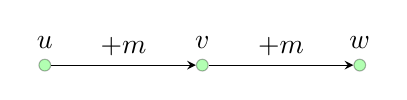
\begin{tikzpicture}
                \node[circle, draw, inner sep=1.5pt, fill=green, opacity=0.3, label={90:$u$}] (u) at (0, 0) {};
                \node[circle, draw, inner sep=1.5pt, fill=green, opacity=0.3, label={90:$v$}] (v) at (2, 0.0) {};
                \node[circle, draw, inner sep=1.5pt, fill=green, opacity=0.3, label={90:$w$}] (w) at (4, 0.0) {};

                \draw[-stealth] (u) -- node[above] {$+m$} (v);
                \draw[-stealth] (v) -- node[above] {$+m$} (w);
            \end{tikzpicture}
        \end{figure}
        \noindent So, the incoming flow and the outgoing flow for $v$ increases by $m$, so given that the flow was conserved for $v$ originally, it is still conserved.

        \item if we have a forwards-edge and a backwards-edge, then the edges in $E$ are $(u, v)$ and $(w, v)$, as given below:
        \begin{figure}[H]
            \centering
            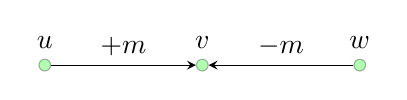
\begin{tikzpicture}
                \node[circle, draw, inner sep=1.5pt, fill=green, opacity=0.3, label={90:$u$}] (u) at (0, 0) {};
                \node[circle, draw, inner sep=1.5pt, fill=green, opacity=0.3, label={90:$v$}] (v) at (2, 0.0) {};
                \node[circle, draw, inner sep=1.5pt, fill=green, opacity=0.3, label={90:$w$}] (w) at (4, 0.0) {};

                \draw[-stealth] (u) -- node[above] {$+m$} (v);
                \draw[-stealth] (w) -- node[above] {$-m$} (v);
            \end{tikzpicture}
        \end{figure}
        \noindent By the edge $(u, v)$, the flow increases by $m$; by the edge $(w, v)$, the flow decreases by $m$. Hence, the incoming flow for $v$ doesn't change, i.e. it is still conserved.
    \end{itemize}
    We can use the same idea for the other two cases. So, the flow is conserved in each case. We have also seen above that the value of the new flow $f'$ is $m > 0$ more than the value of the flow $f$. Hence, $f$ is not a maximum flow.

    To prove the other direction, we introduce the concept of a cut. A \emph{cut} in a network is a set of edges in $E$ such that removing those edges means we no longer have a path from the source to the sink. For example, consider the following network:
    \begin{figure}[H]
        \centering
        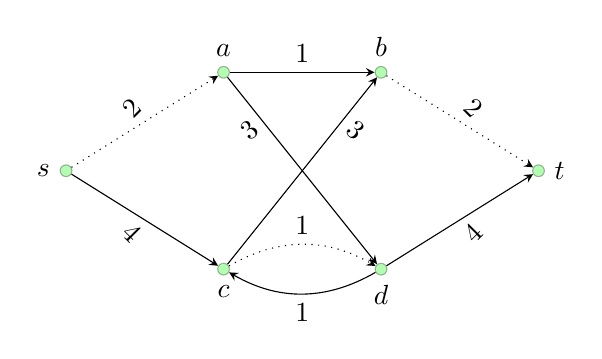
\begin{tikzpicture}
            \node[circle, draw, inner sep=1.5pt, fill=green, opacity=0.3, label={-180:$s$}] (s) at (0, 0) {};
            \node[circle, draw, inner sep=1.5pt, fill=green, opacity=0.3, label={90:$a$}] (a) at (2, 1.25) {};
            \node[circle, draw, inner sep=1.5pt, fill=green, opacity=0.3, label={90:$b$}] (b) at (4, 1.25) {};
            \node[circle, draw, inner sep=1.5pt, fill=green, opacity=0.3, label={-90:$c$}] (c) at (2, -1.25) {};
            \node[circle, draw, inner sep=1.5pt, fill=green, opacity=0.3, label={-90:$d$}] (d) at (4, -1.25) {};
            \node[circle, draw, inner sep=1.5pt, fill=green, opacity=0.3, label={0:$t$}] (t) at (6, 0) {};

            \draw[-stealth, dotted] (s) -- node[above, rotate=45] {2} (a);
            \draw[-stealth] (s) -- node[below, rotate=-45] {4} (c);
            \draw[-stealth] (a) -- node[above] {1} (b);
            \draw[-stealth, dotted] (b) -- node[above, rotate=-45] {2} (t);
            \draw[-stealth] (d) -- node[below, rotate=45] {4} (t);
            \draw[-stealth] (a) -- node[below left, rotate=40, pos=0.15] {3} (d);
            \draw[-stealth] (c) -- node[below right, rotate=-40, pos=0.85] {3} (b);
            \draw[-stealth, dotted] (c) edge[bend left] node[above] {1} (d);
            \draw[-stealth] (d) edge[bend left] node[below] {1} (c);
        \end{tikzpicture}
    \end{figure}
    \noindent The values given for each edge represents its capacity. In the graph above, if we remove the dotted edges, then we can no longer travel from the source $s$ to the sink $t$- we get stuck at $b$. We can also define cuts in a different way- consider a partition of the vertex set into the sets $A$ and $B$, where the source $s \in A$ and the sink $t \in B$. We can define a cut as follows:
    \[C = A \times B \cap E = \{(u, v) \in E \mid u \in A, v \in B\}.\]
    In the graph above, the cut $C$ has $A = \{s, b, c\}$ and $B = \{t, a, d\}$. We define the capacity of a cut $C$ by the sum of the capacity of the edges in it. So, in the example above, we have $\operatorname{cap}(C) = 5$.

    % We can show that the two definitions of the cut are equivalent. We will show one direction- if we remove the edges at the cut $C$, then there is no path from the source to the sink. Assume, for a contradiction, that there is a path from the source to the sink. Denote the path as follows: $(s, e_1), (e_1, e_2), \dots, (e_r, t)$. We know that $s \in A$. Since $(s, e_1)$ remains in the graph, the edge cannot be in $C$. Hence, $e_1 \in A$. Using this argument inductively, we find that $e_r \in A$. This would imply that $t \in A$. However, we must have $t \in B$. This is a contradiction. So, there is no path from the source to the sink.

    We now return to the proof of the Augmenting Path Theorem. In particular, we want to show that if a network has no augmenting path, then it is a maximum flow. We do this by constructing a cut with capacity equal to the capacity of the network flow. Then, we can make use of the Max-Flox Min-Cut theorem\sidefootnote{The Max-Flow Min-Cut theorem states that the value of a maximum flow is equal to the capacity of a minimum cut.}  to show that the network flow has maximum capacity. Intuitively, this follows since the cut ensures that no addition flow can pass from the source to the sink, hence the current flow is maximal.

    Let $G = (V, E)$ be the network, with source $s$ and sink $t$. We define a \emph{partial augmenting path} to be a path that is like an augmenting path, but does not end at the sink. Let $A \subseteq V$ be the set of partial augmenting paths and $B = V \setminus A$. We know that there is no augmenting path in $G$, so we know that $t \not\in A$, i.e. $t \in B$. Furthermore, the trivial path gives us $s \in A$. So, we define the cut as follows:
    \[C = \{(u, v) \in E \mid u \in A, v \in B\}.\]
    For an edge $(u, v) \in C$ with $(u, v) \in E$, we claim that the flow $f(u, v)$ equals capacity- otherwise, we can get a valid edge from $u$ to $v$, which gives us a partial augmenting path, i.e. $v \in A$. Similarly, for $(u, v) \in C$ with $(v, u) \in E$, we claim that the flow $f(v, u) = 0$- we get the same contradiction otherwise. This implies that the capacity of the cut equals the capacity of the flow, so the flow is maximum. 

    Above, we saw that the following is a maximum network flow:
    \begin{figure}[H]
        \centering
        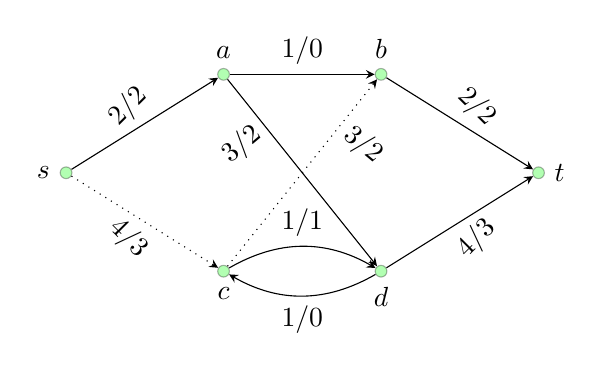
\begin{tikzpicture}
            \node[circle, draw, inner sep=1.5pt, fill=green, opacity=0.3, label={-180:$s$}] (s) at (0, 0) {};
            \node[circle, draw, inner sep=1.5pt, fill=green, opacity=0.3, label={90:$a$}] (a) at (2, 1.25) {};
            \node[circle, draw, inner sep=1.5pt, fill=green, opacity=0.3, label={90:$b$}] (b) at (4, 1.25) {};
            \node[circle, draw, inner sep=1.5pt, fill=green, opacity=0.3, label={-90:$c$}] (c) at (2, -1.25) {};
            \node[circle, draw, inner sep=1.5pt, fill=green, opacity=0.3, label={-90:$d$}] (d) at (4, -1.25) {};
            \node[circle, draw, inner sep=1.5pt, fill=green, opacity=0.3, label={0:$t$}] (t) at (6, 0) {};

            \draw[-stealth] (s) -- node[above, rotate=45] {2/2} (a);
            \draw[-stealth, dotted] (s) -- node[below, rotate=-45] {4/3} (c);
            \draw[-stealth] (a) -- node[above] {1/0} (b);
            \draw[-stealth] (b) -- node[above, rotate=-45] {2/2} (t);
            \draw[-stealth] (d) -- node[below, rotate=45] {4/3} (t);
            \draw[-stealth] (a) -- node[below left, rotate=40, pos=0.15] {3/2} (d);
            \draw[-stealth, dotted] (c) -- node[below right, rotate=-40, pos=0.85] {3/2} (b);
            \draw[-stealth] (c) edge[bend left] node[above] {1/1} (d);
            \draw[-stealth] (d) edge[bend left] node[below] {1/0} (c);
        \end{tikzpicture}
    \end{figure}
    \noindent The dotted edges give us all the vertices we can reach from $s$. Using this, we can define the partitions $A = \{s, c, b\}$ and $B = \{a, d, t\}$. Then, the cut generated by $A$ and $B$ is the following:
    \begin{figure}[H]
        \centering
        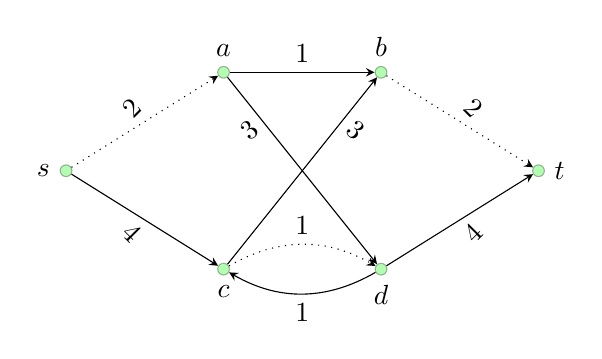
\begin{tikzpicture}
            \node[circle, draw, inner sep=1.5pt, fill=green, opacity=0.3, label={-180:$s$}] (s) at (0, 0) {};
            \node[circle, draw, inner sep=1.5pt, fill=green, opacity=0.3, label={90:$a$}] (a) at (2, 1.25) {};
            \node[circle, draw, inner sep=1.5pt, fill=green, opacity=0.3, label={90:$b$}] (b) at (4, 1.25) {};
            \node[circle, draw, inner sep=1.5pt, fill=green, opacity=0.3, label={-90:$c$}] (c) at (2, -1.25) {};
            \node[circle, draw, inner sep=1.5pt, fill=green, opacity=0.3, label={-90:$d$}] (d) at (4, -1.25) {};
            \node[circle, draw, inner sep=1.5pt, fill=green, opacity=0.3, label={0:$t$}] (t) at (6, 0) {};

            \draw[-stealth, dotted] (s) -- node[above, rotate=45] {2} (a);
            \draw[-stealth] (s) -- node[below, rotate=-45] {4} (c);
            \draw[-stealth] (a) -- node[above] {1} (b);
            \draw[-stealth, dotted] (b) -- node[above, rotate=-45] {2} (t);
            \draw[-stealth] (d) -- node[below, rotate=45] {4} (t);
            \draw[-stealth] (a) -- node[below left, rotate=40, pos=0.15] {3} (d);
            \draw[-stealth] (c) -- node[below right, rotate=-40, pos=0.85] {3} (b);
            \draw[-stealth, dotted] (c) edge[bend left] node[above] {1} (d);
            \draw[-stealth] (d) edge[bend left] node[below] {1} (c);
        \end{tikzpicture}
    \end{figure}
    \noindent The dotted lines show the edges part of the cut. The capacity of this cut is 5, which equals the capacity of the network flow.

    We will now look at the algorithm to find the maximum flow. This is given by the Ford-Fulkerson algorithm. Superficially, the algorithm is the same as for the maximum cardinality matching- we start up with the empty flow and use augmenting paths to increase the flow capacity, until there is no augmenting path.

    We search for augmenting paths using the residual graph. It is a directed weighted graph (not necessarily a network) that we can traverse to find an augmenting path. For instance, we have an example of a flow and its residual graph below.        
    \begin{figure}[H]
        \centering
        \begin{subfigure}{0.48\textwidth}
            \begin{scalebox}{0.8}{
                \centering
                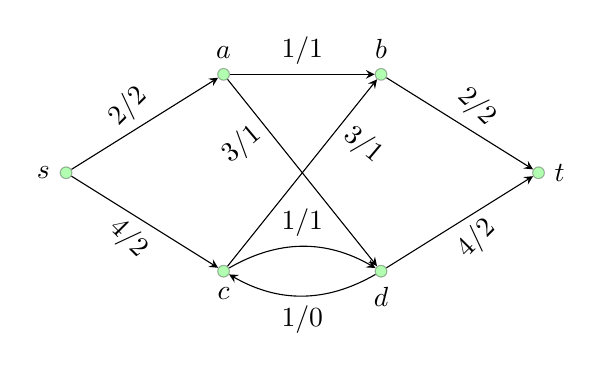
\begin{tikzpicture}
                    \node[circle, draw, inner sep=1.5pt, fill=green, opacity=0.3, label={-180:$s$}] (s) at (0, 0) {};
                    \node[circle, draw, inner sep=1.5pt, fill=green, opacity=0.3, label={90:$a$}] (a) at (2, 1.25) {};
                    \node[circle, draw, inner sep=1.5pt, fill=green, opacity=0.3, label={90:$b$}] (b) at (4, 1.25) {};
                    \node[circle, draw, inner sep=1.5pt, fill=green, opacity=0.3, label={-90:$c$}] (c) at (2, -1.25) {};
                    \node[circle, draw, inner sep=1.5pt, fill=green, opacity=0.3, label={-90:$d$}] (d) at (4, -1.25) {};
                    \node[circle, draw, inner sep=1.5pt, fill=green, opacity=0.3, label={0:$t$}] (t) at (6, 0) {};

                    \draw[-stealth] (s) -- node[above, rotate=45] {2/2} (a);
                    \draw[-stealth] (s) -- node[below, rotate=-45] {4/2} (c);
                    \draw[-stealth] (a) -- node[above] {1/1} (b);
                    \draw[-stealth] (b) -- node[above, rotate=-45] {2/2} (t);
                    \draw[-stealth] (d) -- node[below, rotate=45] {4/2} (t);
                    \draw[-stealth] (a) -- node[below left, rotate=40, pos=0.15] {3/1} (d);
                    \draw[-stealth] (c) -- node[below right, rotate=-40, pos=0.85] {3/1} (b);
                    \draw[-stealth] (c) edge[bend left] node[above] {1/1} (d);
                    \draw[-stealth] (d) edge[bend left] node[below] {1/0} (c);
                \end{tikzpicture}
                }
            \end{scalebox}
        \end{subfigure}
        \hfill
        \begin{subfigure}{0.48\textwidth}
            \begin{scalebox}{0.8}{
                \centering
                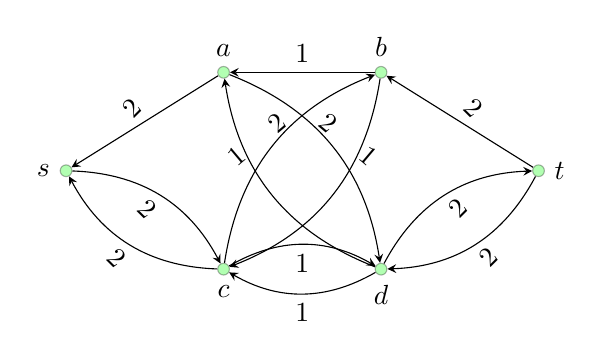
\begin{tikzpicture}
                    \node[circle, draw, inner sep=1.5pt, fill=green, opacity=0.3, label={-180:$s$}] (s) at (0, 0) {};
                    \node[circle, draw, inner sep=1.5pt, fill=green, opacity=0.3, label={90:$a$}] (a) at (2, 1.25) {};
                    \node[circle, draw, inner sep=1.5pt, fill=green, opacity=0.3, label={90:$b$}] (b) at (4, 1.25) {};
                    \node[circle, draw, inner sep=1.5pt, fill=green, opacity=0.3, label={-90:$c$}] (c) at (2, -1.25) {};
                    \node[circle, draw, inner sep=1.5pt, fill=green, opacity=0.3, label={-90:$d$}] (d) at (4, -1.25) {};
                    \node[circle, draw, inner sep=1.5pt, fill=green, opacity=0.3, label={0:$t$}] (t) at (6, 0) {};

                    \draw[-stealth] (a) -- node[above, rotate=45] {2} (s);
                    \draw[-stealth] (s) edge[bend left] node[below, rotate=-45] {2} (c);
                    \draw[-stealth] (c) edge[bend left] node[below, rotate=-45] {2} (s);
                    \draw[-stealth] (b) -- node[above] {1} (a);
                    \draw[-stealth] (t) -- node[above, rotate=-45] {2} (b);
                    \draw[-stealth] (d) edge[bend left] node[below, rotate=45] {2} (t);
                    \draw[-stealth] (t) edge[bend left] node[below, rotate=45] {2} (d);
                    \draw[-stealth] (a) edge[bend left] node[below left, rotate=40, pos=0.2] {2} (d);
                    \draw[-stealth] (d) edge[bend left] node[below left, rotate=40, pos=0.8] {1} (a);
                    \draw[-stealth] (c) edge[bend left] node[below right, rotate=-40, pos=0.8] {2} (b);
                    \draw[-stealth] (b) edge[bend left] node[below right, rotate=-40, pos=0.2] {1} (c);
                    \draw[-stealth] (d) edge[bend left] node[below] {1} (c);
                    \draw[-stealth] (c) edge[bend left] node[below] {1} (d);
                \end{tikzpicture}
                }
            \end{scalebox}
        \end{subfigure}
    \end{figure}
    \noindent The vertex set in the network and the residue graph is identical. For an edge $(u, v) \in E$, if its flow $f(u, v)$ is smaller than the capacity $c(u, v)$, then there is an edge $(u, v)$ in the residue with weight equal to the slack. Also, if the flow $f(u, v)$ is greater than zero, then there is an edge $(v, u)$ in the residue with weight equal to the flow. In the case above, there are 2 ways we can get the edge $(d, c)$ in the residual graph- a forwards-edge and a backwards-edge. This can be represented in many ways- the flow can be equal to one of them, the sum of them, or be represented by multiple edges. We shall always choose one of them.

    To find an augmenting path, we traverse the residue path, starting from the source and ending up at the sink. We can use an algorithm such as depth-first search or breadth-first search to find the path. The edges that are part of the path will lead to an augmenting path. We illustrate this with the network/residue above.
    \begin{figure}[H]
        \centering
        \begin{subfigure}{0.45\textwidth}
            \begin{scalebox}{0.8}{
                \centering
                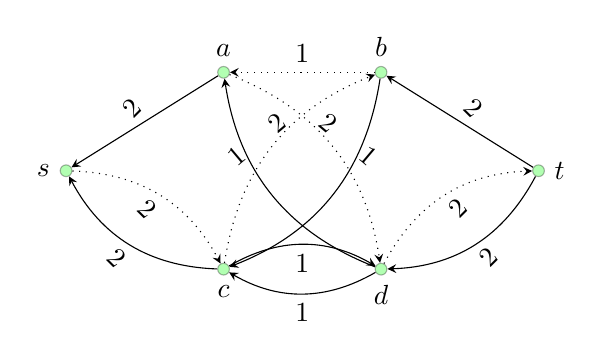
\begin{tikzpicture}
                    \node[circle, draw, inner sep=1.5pt, fill=green, opacity=0.3, label={-180:$s$}] (s) at (0, 0) {};
                    \node[circle, draw, inner sep=1.5pt, fill=green, opacity=0.3, label={90:$a$}] (a) at (2, 1.25) {};
                    \node[circle, draw, inner sep=1.5pt, fill=green, opacity=0.3, label={90:$b$}] (b) at (4, 1.25) {};
                    \node[circle, draw, inner sep=1.5pt, fill=green, opacity=0.3, label={-90:$c$}] (c) at (2, -1.25) {};
                    \node[circle, draw, inner sep=1.5pt, fill=green, opacity=0.3, label={-90:$d$}] (d) at (4, -1.25) {};
                    \node[circle, draw, inner sep=1.5pt, fill=green, opacity=0.3, label={0:$t$}] (t) at (6, 0) {};

                    \draw[-stealth] (a) -- node[above, rotate=45] {2} (s);
                    \draw[-stealth, dotted] (s) edge[bend left] node[below, rotate=-45] {2} (c);
                    \draw[-stealth] (c) edge[bend left] node[below, rotate=-45] {2} (s);
                    \draw[-stealth, dotted] (b) -- node[above] {1} (a);
                    \draw[-stealth] (t) -- node[above, rotate=-45] {2} (b);
                    \draw[-stealth, dotted] (d) edge[bend left] node[below, rotate=45] {2} (t);
                    \draw[-stealth] (t) edge[bend left] node[below, rotate=45] {2} (d);
                    \draw[-stealth, dotted] (a) edge[bend left] node[below left, rotate=40, pos=0.2] {2} (d);
                    \draw[-stealth] (d) edge[bend left] node[below left, rotate=40, pos=0.8] {1} (a);
                    \draw[-stealth, dotted] (c) edge[bend left] node[below right, rotate=-40, pos=0.8] {2} (b);
                    \draw[-stealth] (b) edge[bend left] node[below right, rotate=-40, pos=0.2] {1} (c);
                    \draw[-stealth] (d) edge[bend left] node[below] {1} (c);
                    \draw[-stealth] (c) edge[bend left] node[below] {1} (d);
                \end{tikzpicture}
                }
            \end{scalebox}
        \end{subfigure}
        \hfill
        \begin{subfigure}{0.45\textwidth}
            \centering
            \begin{scalebox}{0.8}{
                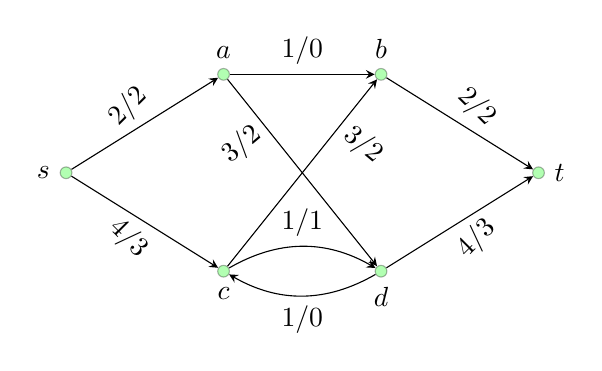
\begin{tikzpicture}
                    \node[circle, draw, inner sep=1.5pt, fill=green, opacity=0.3, label={-180:$s$}] (s) at (0, 0) {};
                    \node[circle, draw, inner sep=1.5pt, fill=green, opacity=0.3, label={90:$a$}] (a) at (2, 1.25) {};
                    \node[circle, draw, inner sep=1.5pt, fill=green, opacity=0.3, label={90:$b$}] (b) at (4, 1.25) {};
                    \node[circle, draw, inner sep=1.5pt, fill=green, opacity=0.3, label={-90:$c$}] (c) at (2, -1.25) {};
                    \node[circle, draw, inner sep=1.5pt, fill=green, opacity=0.3, label={-90:$d$}] (d) at (4, -1.25) {};
                    \node[circle, draw, inner sep=1.5pt, fill=green, opacity=0.3, label={0:$t$}] (t) at (6, 0) {};
        
                    \draw[-stealth] (s) -- node[above, rotate=45] {2/2} (a);
                    \draw[-stealth] (s) -- node[below, rotate=-45] {4/3} (c);
                    \draw[-stealth] (a) -- node[above] {1/0} (b);
                    \draw[-stealth] (b) -- node[above, rotate=-45] {2/2} (t);
                    \draw[-stealth] (d) -- node[below, rotate=45] {4/3} (t);
                    \draw[-stealth] (a) -- node[below left, rotate=40, pos=0.15] {3/2} (d);
                    \draw[-stealth] (c) -- node[below right, rotate=-40, pos=0.85] {3/2} (b);
                    \draw[-stealth] (c) edge[bend left] node[above] {1/1} (d);
                    \draw[-stealth] (d) edge[bend left] node[below] {1/0} (c);
                \end{tikzpicture}
                }
            \end{scalebox}
        \end{subfigure}
    \end{figure}
    \noindent The path in the residual graph is given on the left- it is: $(s, c)$, $(c, b)$, $(b, a)$, $(a, d)$ and $(d, t)$. This is an augmented path in the network. Using this augmented path, we can improve the flow. In this case, we increase the capacity by 1- this is given on the right.

    Below is the Ford-Fulkerson algorithm:
\begin{lstlisting}[language=pseudocode]
void fordFulkerson(Network network) {
    Graph graph = network.residue;
    List<Edge> edges = graph.augmentingPath;
    while (edges.isNotEmpty) {
        int m = edges.minVal;
        network.augment(edges, m);
        edges = graph.augmentingPath;
    }
}
\end{lstlisting}
    We assume that the network is initialised with flow equal to 0. The \texttt{augment} method changes the flow of an edge by $m$- a forwards-edge has its flow increased, while a backwards-edge has its flow decreased. We can find out whether an edge is a forwards-edge or a backwards-edge by checking whether it can be increased/decreased by $m$; we can also keep track of this using a boolean field.

    We will now consider the complexity of the algorithm. The initialisation is $O(|E|)$- we set the flow 0 to all the edges. The main loop iterates at most $O(\texttt{maxFlow})$ times (if the flow only ever increases by 1). To build the residual graph, it takes $O(|V| + |E|)$ time- we have the same number of vertices and (at most) double the edges. We can find an augmenting path in $O(|V| + |E|)$ time, e.g. using BFS or DFS. The augmentation changes the flow of the edges- it takes $O(|E|)$ time. If we assume that every vertex is on a directed path from $s$ to $t$, we find that $|V| = O(|E|)$. Hence, the algorithm has complexity $O(|E| \cdot \texttt{maxFlow})$. This is a pseudo-linear algorithm, which can be quite inefficient.

    The bound of \texttt{maxFlow} can be improved in some cases by choosing the right augmenting path. For example, consider the following network, with the given capacities:
    \begin{figure}[H]
        \centering
        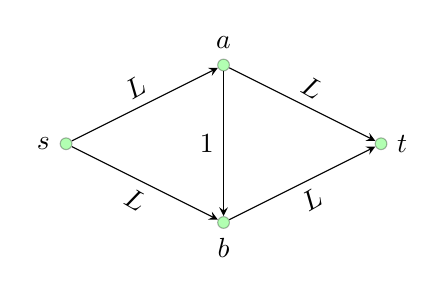
\begin{tikzpicture}
            \node[circle, draw, inner sep=1.5pt, fill=green, opacity=0.3, label={180:$s$}] (s) at (0, 0) {};
            \node[circle, draw, inner sep=1.5pt, fill=green, opacity=0.3, label={90:$a$}] (a) at (2, 1) {};
            \node[circle, draw, inner sep=1.5pt, fill=green, opacity=0.3, label={-90:$b$}] (b) at (2, -1) {};
            \node[circle, draw, inner sep=1.5pt, fill=green, opacity=0.3, label={0:$t$}] (t) at (4, 0) {};
            
            \draw[-stealth] (s) --  node[above, rotate=30] {$L$} (a);
            \draw[-stealth] (s) --  node[below, rotate=-30] {$L$} (b);
            \draw[-stealth] (a) -- node[above, rotate=-30] {$L$} (t);
            \draw[-stealth] (b) -- node[below, rotate=30] {$L$} (t);
            \draw[-stealth] (a) -- node[left] {1} (b);
        \end{tikzpicture}
    \end{figure}
    \noindent If we choose the path $(s, a), (a, b), (b, t)$, then we can only increase the capacity by 1. We can then choose the path $(s, b), (b, a), (a, t)$, the same thing happens. The algorithm might loop around these two choices, and only find the maximum flow after $2L$ iterations. However, we can find the maximum flow in just 2 iterations- take the edges $(s, a), (a, t)$ and $(s, b), (b, t)$. 
    
    We can get this improvement by always choosing the shortest augmenting path. This can be achieved using breadth-first search. If we use this version of the Ford-Fulkerson algorithm, then we are using the \emph{Edomons-Karp heuristic}. Using this version, we only search for an augmenting path $O(|V||E|)$ times, so the Ford-Fulkerson algorithm has complexity $O(|V||E|^2) = O(|E|^3)$. The fastest algorithm known has complexity $O(|V||E|)$.

    % \begin{figure}[H]
    %     \centering
    %     \begin{tikzpicture}
    %         \node[circle, draw, inner sep=1.5pt, fill=green, opacity=0.3, label={-180:$s$}] (s) at (0, 0) {};
    %         \node[circle, draw, inner sep=1.5pt, fill=green, opacity=0.3, label={90:$a$}] (a) at (2, 1.25) {};
    %         \node[circle, draw, inner sep=1.5pt, fill=green, opacity=0.3, label={90:$b$}] (b) at (4, 1.25) {};
    %         \node[circle, draw, inner sep=1.5pt, fill=green, opacity=0.3, label={-90:$c$}] (c) at (2, -1.25) {};
    %         \node[circle, draw, inner sep=1.5pt, fill=green, opacity=0.3, label={-90:$d$}] (d) at (4, -1.25) {};
    %         \node[circle, draw, inner sep=1.5pt, fill=green, opacity=0.3, label={0:$t$}] (t) at (6, 0) {};

    %         \draw[-stealth] (a) -- node[above, rotate=45] {2} (s);
    %         \draw[-stealth, dotted] (s) edge[bend left] node[below, rotate=-45] {1} (c);
    %         \draw[-stealth] (c) edge[bend left] node[below, rotate=-45] {3} (s);
    %         \draw[-stealth] (a) -- node[above] {1} (b);
    %         \draw[-stealth] (t) -- node[above, rotate=-45] {2} (b);
    %         \draw[-stealth] (d) edge[bend left] node[below, rotate=45] {1} (t);
    %         \draw[-stealth] (t) edge[bend left] node[below, rotate=45] {3} (d);
    %         \draw[-stealth] (a) edge[bend left] node[below left, rotate=40, pos=0.2] {1} (d);
    %         \draw[-stealth] (d) edge[bend left] node[below left, rotate=40, pos=0.8] {2} (a);
    %         \draw[-stealth, dotted] (c) edge[bend left] node[below right, rotate=-40, pos=0.8] {1} (b);
    %         \draw[-stealth] (b) edge[bend left] node[below right, rotate=-40, pos=0.2] {2} (c);
    %         \draw[-stealth] (d) edge[bend left] node[below] {1} (c);
    %         \draw[-stealth] (c) edge[bend left] node[below] {1} (d);
    %     \end{tikzpicture}
    % \end{figure}
    % TODO: 3600 onwards
    
    We will now illustrate how the algorithm works with an example. Assume we have the following network, with the given capacities:
    \begin{figure}[H]
        \centering
        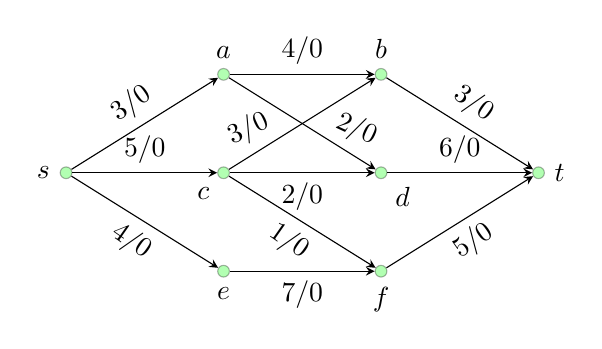
\begin{tikzpicture}
            \node[circle, draw, inner sep=1.5pt, fill=green, opacity=0.3, label={-180:$s$}] (s) at (0, 0) {};
            \node[circle, draw, inner sep=1.5pt, fill=green, opacity=0.3, label={90:$a$}] (a) at (2, 1.25) {};
            \node[circle, draw, inner sep=1.5pt, fill=green, opacity=0.3, label={90:$b$}] (b) at (4, 1.25) {};
            \node[circle, draw, inner sep=1.5pt, fill=green, opacity=0.3, label={-135:$c$}] (c) at (2, 0) {};
            \node[circle, draw, inner sep=1.5pt, fill=green, opacity=0.3, label={-45:$d$}] (d) at (4, 0) {};
            \node[circle, draw, inner sep=1.5pt, fill=green, opacity=0.3, label={-90:$e$}] (e) at (2, -1.25) {};
            \node[circle, draw, inner sep=1.5pt, fill=green, opacity=0.3, label={-90:$f$}] (f) at (4, -1.25) {};
            \node[circle, draw, inner sep=1.5pt, fill=green, opacity=0.3, label={0:$t$}] (t) at (6, 0) {};

            \draw[-stealth] (s) -- node[above, rotate=35] {$3/0$} (a);
            \draw[-stealth] (s) -- node[above] {$5/0$} (c);
            \draw[-stealth] (s) -- node[below, rotate=-35] {$4/0$} (e);
            \draw[-stealth] (a) -- node[above] {$4/0$} (b);
            \draw[-stealth] (e) -- node[below] {$7/0$} (f);
            \draw[-stealth] (b) -- node[above, rotate=-35] {$3/0$} (t);
            \draw[-stealth] (d) -- node[above] {$6/0$} (t);
            \draw[-stealth] (f) -- node[below, rotate=35] {$5/0$} (t);
            \draw[-stealth] (c) -- node[below] {$2/0$} (d);
            \draw[-stealth] (a) -- node[above, rotate=-25, pos=0.8] {$2/0$} (d);
            \draw[-stealth] (c) -- node[above, rotate=25, pos=0.2] {$3/0$} (b);
            \draw[-stealth] (c) -- node[below, rotate=-35] {$1/0$} (f);
        \end{tikzpicture}
    \end{figure}
    \noindent We initialise the flow with value 0, and construct the residual graph.
    \begin{figure}[H]
        \centering
        \begin{subfigure}{0.48\textwidth}
            \centering
            \scalebox{0.8}{
                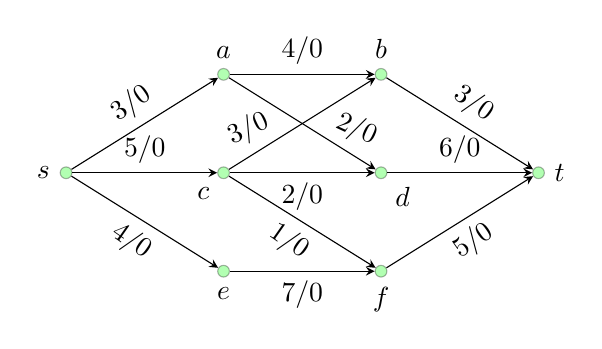
\begin{tikzpicture}
                    \node[circle, draw, inner sep=1.5pt, fill=green, opacity=0.3, label={-180:$s$}] (s) at (0, 0) {};
                    \node[circle, draw, inner sep=1.5pt, fill=green, opacity=0.3, label={90:$a$}] (a) at (2, 1.25) {};
                    \node[circle, draw, inner sep=1.5pt, fill=green, opacity=0.3, label={90:$b$}] (b) at (4, 1.25) {};
                    \node[circle, draw, inner sep=1.5pt, fill=green, opacity=0.3, label={-135:$c$}] (c) at (2, 0) {};
                    \node[circle, draw, inner sep=1.5pt, fill=green, opacity=0.3, label={-45:$d$}] (d) at (4, 0) {};
                    \node[circle, draw, inner sep=1.5pt, fill=green, opacity=0.3, label={-90:$e$}] (e) at (2, -1.25) {};
                    \node[circle, draw, inner sep=1.5pt, fill=green, opacity=0.3, label={-90:$f$}] (f) at (4, -1.25) {};
                    \node[circle, draw, inner sep=1.5pt, fill=green, opacity=0.3, label={0:$t$}] (t) at (6, 0) {};

                    \draw[-stealth] (s) -- node[above, rotate=35] {$3/0$} (a);
                    \draw[-stealth] (s) -- node[above] {$5/0$} (c);
                    \draw[-stealth] (s) -- node[below, rotate=-35] {$4/0$} (e);
                    \draw[-stealth] (a) -- node[above] {$4/0$} (b);
                    \draw[-stealth] (e) -- node[below] {$7/0$} (f);
                    \draw[-stealth] (b) -- node[above, rotate=-35] {$3/0$} (t);
                    \draw[-stealth] (d) -- node[above] {$6/0$} (t);
                    \draw[-stealth] (f) -- node[below, rotate=35] {$5/0$} (t);
                    \draw[-stealth] (c) -- node[below] {$2/0$} (d);
                    \draw[-stealth] (a) -- node[above, rotate=-25, pos=0.8] {$2/0$} (d);
                    \draw[-stealth] (c) -- node[above, rotate=25, pos=0.2] {$3/0$} (b);
                    \draw[-stealth] (c) -- node[below, rotate=-35] {$1/0$} (f);
                \end{tikzpicture}
            }
        \end{subfigure}
        \hfill
        \begin{subfigure}{0.48\textwidth}
            \centering
            \scalebox{0.8}{
                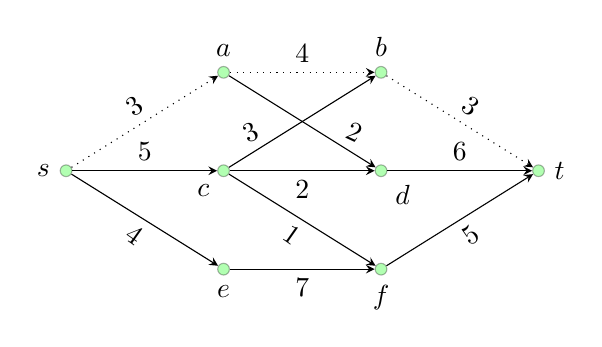
\begin{tikzpicture}
                    \node[circle, draw, inner sep=1.5pt, fill=green, opacity=0.3, label={-180:$s$}] (s) at (0, 0) {};
                    \node[circle, draw, inner sep=1.5pt, fill=green, opacity=0.3, label={90:$a$}] (a) at (2, 1.25) {};
                    \node[circle, draw, inner sep=1.5pt, fill=green, opacity=0.3, label={90:$b$}] (b) at (4, 1.25) {};
                    \node[circle, draw, inner sep=1.5pt, fill=green, opacity=0.3, label={-135:$c$}] (c) at (2, 0) {};
                    \node[circle, draw, inner sep=1.5pt, fill=green, opacity=0.3, label={-45:$d$}] (d) at (4, 0) {};
                    \node[circle, draw, inner sep=1.5pt, fill=green, opacity=0.3, label={-90:$e$}] (e) at (2, -1.25) {};
                    \node[circle, draw, inner sep=1.5pt, fill=green, opacity=0.3, label={-90:$f$}] (f) at (4, -1.25) {};
                    \node[circle, draw, inner sep=1.5pt, fill=green, opacity=0.3, label={0:$t$}] (t) at (6, 0) {};

                    \draw[-stealth, dotted] (s) -- node[above, rotate=35] {$3$} (a);
                    \draw[-stealth] (s) -- node[above] {$5$} (c);
                    \draw[-stealth] (s) -- node[below, rotate=-35] {$4$} (e);
                    \draw[-stealth, dotted] (a) -- node[above] {$4$} (b);
                    \draw[-stealth] (e) -- node[below] {$7$} (f);
                    \draw[-stealth, dotted] (b) -- node[above, rotate=-35] {$3$} (t);
                    \draw[-stealth] (d) -- node[above] {$6$} (t);
                    \draw[-stealth] (f) -- node[below, rotate=35] {$5$} (t);
                    \draw[-stealth] (c) -- node[below] {$2$} (d);
                    \draw[-stealth] (a) -- node[above, rotate=-25, pos=0.8] {$2$} (d);
                    \draw[-stealth] (c) -- node[above, rotate=25, pos=0.2] {$3$} (b);
                    \draw[-stealth] (c) -- node[below, rotate=-35] {$1$} (f);
                \end{tikzpicture}
            }
        \end{subfigure}
    \end{figure}
    \noindent Note that at the start, the residual graph only has forwards-edges of full capacity- the flow is 0, so we have no backwards edge, and we just have a forwards edge equal to the slack. The dotted path on the right shows the (shortest) path on the residual graph. This is an augmenting path in the network, which we use to increase the flow to 3.
    \begin{figure}[H]
        \centering
        \begin{subfigure}{0.48\textwidth}
            \centering
            \scalebox{0.8}{
                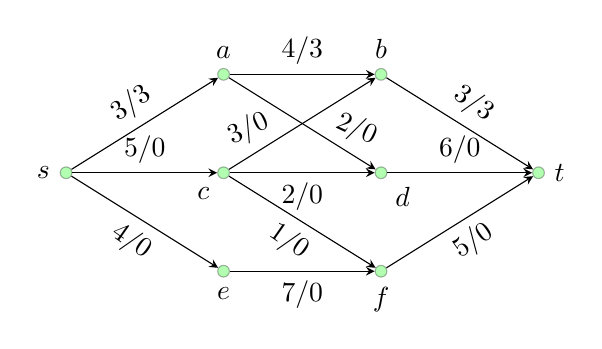
\begin{tikzpicture}
                    \node[circle, draw, inner sep=1.5pt, fill=green, opacity=0.3, label={-180:$s$}] (s) at (0, 0) {};
                    \node[circle, draw, inner sep=1.5pt, fill=green, opacity=0.3, label={90:$a$}] (a) at (2, 1.25) {};
                    \node[circle, draw, inner sep=1.5pt, fill=green, opacity=0.3, label={90:$b$}] (b) at (4, 1.25) {};
                    \node[circle, draw, inner sep=1.5pt, fill=green, opacity=0.3, label={-135:$c$}] (c) at (2, 0) {};
                    \node[circle, draw, inner sep=1.5pt, fill=green, opacity=0.3, label={-45:$d$}] (d) at (4, 0) {};
                    \node[circle, draw, inner sep=1.5pt, fill=green, opacity=0.3, label={-90:$e$}] (e) at (2, -1.25) {};
                    \node[circle, draw, inner sep=1.5pt, fill=green, opacity=0.3, label={-90:$f$}] (f) at (4, -1.25) {};
                    \node[circle, draw, inner sep=1.5pt, fill=green, opacity=0.3, label={0:$t$}] (t) at (6, 0) {};

                    \draw[-stealth] (s) -- node[above, rotate=35] {$3/3$} (a);
                    \draw[-stealth] (s) -- node[above] {$5/0$} (c);
                    \draw[-stealth] (s) -- node[below, rotate=-35] {$4/0$} (e);
                    \draw[-stealth] (a) -- node[above] {$4/3$} (b);
                    \draw[-stealth] (e) -- node[below] {$7/0$} (f);
                    \draw[-stealth] (b) -- node[above, rotate=-35] {$3/3$} (t);
                    \draw[-stealth] (d) -- node[above] {$6/0$} (t);
                    \draw[-stealth] (f) -- node[below, rotate=35] {$5/0$} (t);
                    \draw[-stealth] (c) -- node[below] {$2/0$} (d);
                    \draw[-stealth] (a) -- node[above, rotate=-25, pos=0.8] {$2/0$} (d);
                    \draw[-stealth] (c) -- node[above, rotate=25, pos=0.2] {$3/0$} (b);
                    \draw[-stealth] (c) -- node[below, rotate=-35] {$1/0$} (f);
                \end{tikzpicture}
            }
        \end{subfigure}
        \hfill
        \begin{subfigure}{0.48\textwidth}
            \centering
            \scalebox{0.8}{
                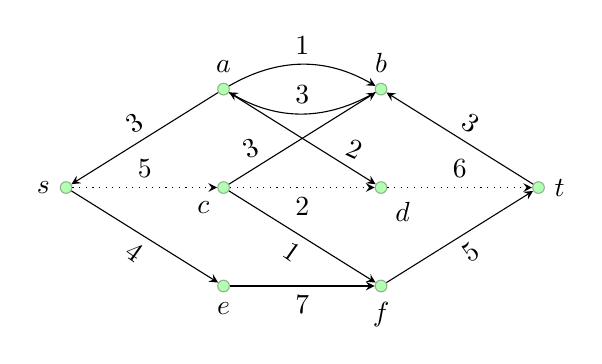
\begin{tikzpicture}
                    \node[circle, draw, inner sep=1.5pt, fill=green, opacity=0.3, label={-180:$s$}] (s) at (0, 0) {};
                    \node[circle, draw, inner sep=1.5pt, fill=green, opacity=0.3, label={90:$a$}] (a) at (2, 1.25) {};
                    \node[circle, draw, inner sep=1.5pt, fill=green, opacity=0.3, label={90:$b$}] (b) at (4, 1.25) {};
                    \node[circle, draw, inner sep=1.5pt, fill=green, opacity=0.3, label={-135:$c$}] (c) at (2, 0) {};
                    \node[circle, draw, inner sep=1.5pt, fill=green, opacity=0.3, label={-45:$d$}] (d) at (4, 0) {};
                    \node[circle, draw, inner sep=1.5pt, fill=green, opacity=0.3, label={-90:$e$}] (e) at (2, -1.25) {};
                    \node[circle, draw, inner sep=1.5pt, fill=green, opacity=0.3, label={-90:$f$}] (f) at (4, -1.25) {};
                    \node[circle, draw, inner sep=1.5pt, fill=green, opacity=0.3, label={0:$t$}] (t) at (6, 0) {};

                    \draw[-stealth] (a) -- node[above, rotate=35] {$3$} (s);
                    \draw[-stealth, dotted] (s) -- node[above] {$5$} (c);
                    \draw[-stealth] (s) -- node[below, rotate=-35] {$4$} (e);
                    \draw[-stealth] (a) edge[bend left] node[above] {$1$} (b);
                    \draw[-stealth] (b) edge[bend left] node[above] {$3$} (a);
                    \draw[-stealth] (e) -- node[below] {$7$} (f);
                    \draw[-stealth] (t) -- node[above, rotate=-35] {$3$} (b);
                    \draw[-stealth, dotted] (d) -- node[above] {$6$} (t);
                    \draw[-stealth] (f) -- node[below, rotate=35] {$5$} (t);
                    \draw[-stealth, dotted] (c) -- node[below] {$2$} (d);
                    \draw[-stealth] (a) -- node[above, rotate=-25, pos=0.8] {$2$} (d);
                    \draw[-stealth] (c) -- node[above, rotate=25, pos=0.2] {$3$} (b);
                    \draw[-stealth] (c) -- node[below, rotate=-35] {$1$} (f);
                \end{tikzpicture}
            }
        \end{subfigure}
    \end{figure}
    \noindent Typically, when the flow changes, we do not need to re-construct the residual graph; we just modify some edge weights. In this case, the edge $(a, b)$ has its weight reduced to 1, $(s, a)$ flips to $(a, s)$ and so on. We now take the next path in the residue, and augment the network flow using it:
    \begin{figure}[H]
        \centering
        \begin{subfigure}{0.48\textwidth}
            \centering
            \scalebox{0.8}{
                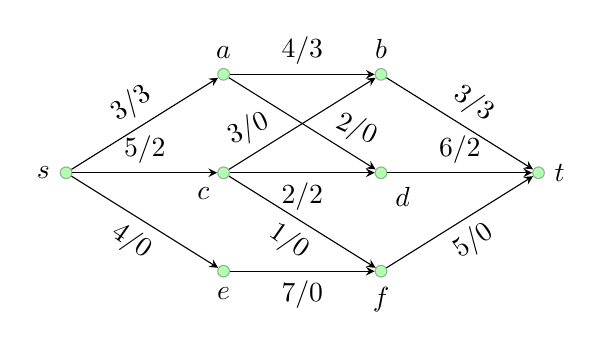
\begin{tikzpicture}
                    \node[circle, draw, inner sep=1.5pt, fill=green, opacity=0.3, label={-180:$s$}] (s) at (0, 0) {};
                    \node[circle, draw, inner sep=1.5pt, fill=green, opacity=0.3, label={90:$a$}] (a) at (2, 1.25) {};
                    \node[circle, draw, inner sep=1.5pt, fill=green, opacity=0.3, label={90:$b$}] (b) at (4, 1.25) {};
                    \node[circle, draw, inner sep=1.5pt, fill=green, opacity=0.3, label={-135:$c$}] (c) at (2, 0) {};
                    \node[circle, draw, inner sep=1.5pt, fill=green, opacity=0.3, label={-45:$d$}] (d) at (4, 0) {};
                    \node[circle, draw, inner sep=1.5pt, fill=green, opacity=0.3, label={-90:$e$}] (e) at (2, -1.25) {};
                    \node[circle, draw, inner sep=1.5pt, fill=green, opacity=0.3, label={-90:$f$}] (f) at (4, -1.25) {};
                    \node[circle, draw, inner sep=1.5pt, fill=green, opacity=0.3, label={0:$t$}] (t) at (6, 0) {};

                    \draw[-stealth] (s) -- node[above, rotate=35] {$3/3$} (a);
                    \draw[-stealth] (s) -- node[above] {$5/2$} (c);
                    \draw[-stealth] (s) -- node[below, rotate=-35] {$4/0$} (e);
                    \draw[-stealth] (a) -- node[above] {$4/3$} (b);
                    \draw[-stealth] (e) -- node[below] {$7/0$} (f);
                    \draw[-stealth] (b) -- node[above, rotate=-35] {$3/3$} (t);
                    \draw[-stealth] (d) -- node[above] {$6/2$} (t);
                    \draw[-stealth] (f) -- node[below, rotate=35] {$5/0$} (t);
                    \draw[-stealth] (c) -- node[below] {$2/2$} (d);
                    \draw[-stealth] (a) -- node[above, rotate=-25, pos=0.8] {$2/0$} (d);
                    \draw[-stealth] (c) -- node[above, rotate=25, pos=0.2] {$3/0$} (b);
                    \draw[-stealth] (c) -- node[below, rotate=-35] {$1/0$} (f);
                \end{tikzpicture}
            }
        \end{subfigure}
        \hfill
        \begin{subfigure}{0.48\textwidth}
            \centering
            \scalebox{0.8}{
                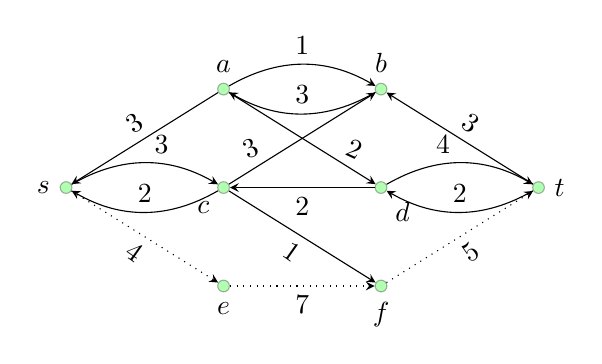
\begin{tikzpicture}
                    \node[circle, draw, inner sep=1.5pt, fill=green, opacity=0.3, label={-180:$s$}] (s) at (0, 0) {};
                    \node[circle, draw, inner sep=1.5pt, fill=green, opacity=0.3, label={90:$a$}] (a) at (2, 1.25) {};
                    \node[circle, draw, inner sep=1.5pt, fill=green, opacity=0.3, label={90:$b$}] (b) at (4, 1.25) {};
                    \node[circle, draw, inner sep=1.5pt, fill=green, opacity=0.3, label={-135:$c$}] (c) at (2, 0) {};
                    \node[circle, draw, inner sep=1.5pt, fill=green, opacity=0.3, label={-45:$d$}] (d) at (4, 0) {};
                    \node[circle, draw, inner sep=1.5pt, fill=green, opacity=0.3, label={-90:$e$}] (e) at (2, -1.25) {};
                    \node[circle, draw, inner sep=1.5pt, fill=green, opacity=0.3, label={-90:$f$}] (f) at (4, -1.25) {};
                    \node[circle, draw, inner sep=1.5pt, fill=green, opacity=0.3, label={0:$t$}] (t) at (6, 0) {};

                    \draw[-stealth] (a) -- node[above, rotate=35] {$3$} (s);
                    \draw[-stealth] (s) edge[bend left] node[above right] {$3$} (c);
                    \draw[-stealth] (c) edge[bend left] node[above] {$2$} (s);
                    \draw[-stealth, dotted] (s) -- node[below, rotate=-35] {$4$} (e);
                    \draw[-stealth] (a) edge[bend left] node[above] {$1$} (b);
                    \draw[-stealth] (b) edge[bend left] node[above] {$3$} (a);
                    \draw[-stealth, dotted] (e) -- node[below] {$7$} (f);
                    \draw[-stealth] (t) -- node[above, rotate=-35] {$3$} (b);
                    \draw[-stealth] (d) edge[bend left] node[above left] {$4$} (t);
                    \draw[-stealth] (t) edge[bend left] node[above] {$2$} (d);
                    \draw[-stealth, dotted] (f) -- node[below, rotate=35] {$5$} (t);
                    \draw[-stealth] (d) -- node[below] {$2$} (c);
                    \draw[-stealth] (a) -- node[above, rotate=-25, pos=0.8] {$2$} (d);
                    \draw[-stealth] (c) -- node[above, rotate=25, pos=0.2] {$3$} (b);
                    \draw[-stealth] (c) -- node[below, rotate=-35] {$1$} (f);
                \end{tikzpicture}
            }
        \end{subfigure}
    \end{figure}
    \noindent We have now increased the network flow value to 5. Using the dotted path (and further paths in the iteration), we can continue improving the capacity of the network until we get the following state:    
    \begin{figure}[H]
        \centering
        \begin{subfigure}{0.48\textwidth}
            \centering
            \scalebox{0.8}{
                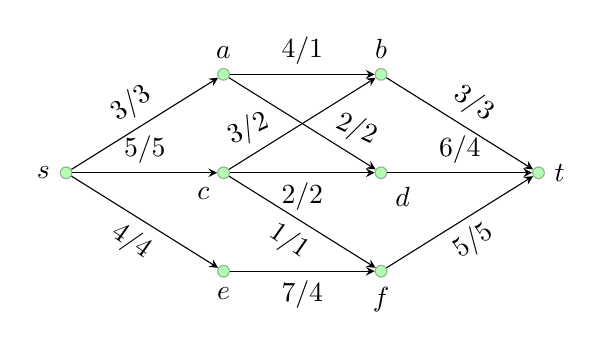
\begin{tikzpicture}
                    \node[circle, draw, inner sep=1.5pt, fill=green, opacity=0.3, label={-180:$s$}] (s) at (0, 0) {};
                    \node[circle, draw, inner sep=1.5pt, fill=green, opacity=0.3, label={90:$a$}] (a) at (2, 1.25) {};
                    \node[circle, draw, inner sep=1.5pt, fill=green, opacity=0.3, label={90:$b$}] (b) at (4, 1.25) {};
                    \node[circle, draw, inner sep=1.5pt, fill=green, opacity=0.3, label={-135:$c$}] (c) at (2, 0) {};
                    \node[circle, draw, inner sep=1.5pt, fill=green, opacity=0.3, label={-45:$d$}] (d) at (4, 0) {};
                    \node[circle, draw, inner sep=1.5pt, fill=green, opacity=0.3, label={-90:$e$}] (e) at (2, -1.25) {};
                    \node[circle, draw, inner sep=1.5pt, fill=green, opacity=0.3, label={-90:$f$}] (f) at (4, -1.25) {};
                    \node[circle, draw, inner sep=1.5pt, fill=green, opacity=0.3, label={0:$t$}] (t) at (6, 0) {};

                    \draw[-stealth] (s) -- node[above, rotate=35] {$3/3$} (a);
                    \draw[-stealth] (s) -- node[above] {$5/5$} (c);
                    \draw[-stealth] (s) -- node[below, rotate=-35] {$4/4$} (e);
                    \draw[-stealth] (a) -- node[above] {$4/1$} (b);
                    \draw[-stealth] (e) -- node[below] {$7/4$} (f);
                    \draw[-stealth] (b) -- node[above, rotate=-35] {$3/3$} (t);
                    \draw[-stealth] (d) -- node[above] {$6/4$} (t);
                    \draw[-stealth] (f) -- node[below, rotate=35] {$5/5$} (t);
                    \draw[-stealth] (c) -- node[below] {$2/2$} (d);
                    \draw[-stealth] (a) -- node[above, rotate=-25, pos=0.8] {$2/2$} (d);
                    \draw[-stealth] (c) -- node[above, rotate=25, pos=0.2] {$3/2$} (b);
                    \draw[-stealth] (c) -- node[below, rotate=-35] {$1/1$} (f);
                \end{tikzpicture}
            }
        \end{subfigure}
        \hfill
        \begin{subfigure}{0.48\textwidth}
            \centering
            \scalebox{0.8}{
                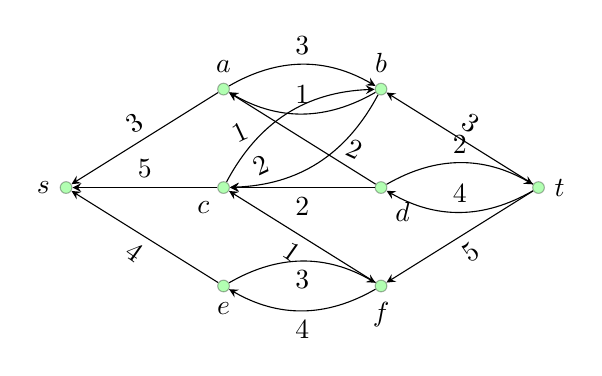
\begin{tikzpicture}
                    \node[circle, draw, inner sep=1.5pt, fill=green, opacity=0.3, label={-180:$s$}] (s) at (0, 0) {};
                    \node[circle, draw, inner sep=1.5pt, fill=green, opacity=0.3, label={90:$a$}] (a) at (2, 1.25) {};
                    \node[circle, draw, inner sep=1.5pt, fill=green, opacity=0.3, label={90:$b$}] (b) at (4, 1.25) {};
                    \node[circle, draw, inner sep=1.5pt, fill=green, opacity=0.3, label={-135:$c$}] (c) at (2, 0) {};
                    \node[circle, draw, inner sep=1.5pt, fill=green, opacity=0.3, label={-45:$d$}] (d) at (4, 0) {};
                    \node[circle, draw, inner sep=1.5pt, fill=green, opacity=0.3, label={-90:$e$}] (e) at (2, -1.25) {};
                    \node[circle, draw, inner sep=1.5pt, fill=green, opacity=0.3, label={-90:$f$}] (f) at (4, -1.25) {};
                    \node[circle, draw, inner sep=1.5pt, fill=green, opacity=0.3, label={0:$t$}] (t) at (6, 0) {};

                    \draw[-stealth] (a) -- node[above, rotate=35] {$3$} (s);
                    \draw[-stealth] (c) -- node[above] {$5$} (s);
                    \draw[-stealth] (e) -- node[below, rotate=-35] {$4$} (s);
                    \draw[-stealth] (a) edge[bend left] node[above] {$3$} (b);
                    \draw[-stealth] (b) edge[bend left] node[above] {$1$} (a);
                    \draw[-stealth] (e) edge[bend left] node[below] {$3$} (f);
                    \draw[-stealth] (f) edge[bend left] node[below] {$4$} (e);
                    \draw[-stealth] (t) -- node[above, rotate=-35] {$3$} (b);
                    \draw[-stealth] (d) edge[bend left] node[above] {$2$} (t);
                    \draw[-stealth] (t) edge[bend left] node[above] {$4$} (d);
                    \draw[-stealth] (t) -- node[below, rotate=35] {$5$} (f);
                    \draw[-stealth] (d) -- node[below] {$2$} (c);
                    \draw[-stealth] (d) -- node[above, rotate=-25, pos=0.2] {$2$} (a);
                    \draw[-stealth] (c) edge[bend left] node[above, rotate=25, pos=0.2] {$1$} (b);
                    \draw[-stealth] (b) edge[bend left] node[above, rotate=25, pos=0.8] {$2$} (c);
                    \draw[-stealth] (f) -- node[below, rotate=-35] {$1$} (c);
                \end{tikzpicture}
            }
        \end{subfigure}
    \end{figure}
    \noindent In the residue graph, the source $s$ has become a sink. Hence, we cannot find a path from the source to the sink $t$. We have found the maximum flow- it has value 12. If we constructed the cut corresponding to this maximum flow, we would find $A = \{s\}$ and $B = \{a, b, c, d, e, f, t\}$. The generated cut is $C = \{(s, a), (s, c), (s, e)\}$, which has value 12. Hence, the Max-Flow Min-Cut theorem tells us that it is a maximum flow.

    We can convert an instance of maximum-cardinality matching to a network flow instance. Let the vertex set be partitioned into left vertices $L$ and right vertices $R$. For every edge $\{u, v\}$, if $u \in L$ and $v \in R$, then the network has a directed edge $(u, v)$. We also have a source $s$, which has edges to every vertex in $L$, and a sink $t$, which has edges from every vertex in $R$. The capacity of each edge in the network is 1. For example, consider the two figures below:
    \begin{figure}[H]
        \centering
        \begin{subfigure}{0.45\textwidth}
            \centering
            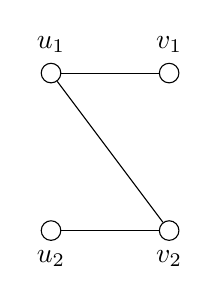
\begin{tikzpicture}
                \node[circle, draw, inner sep=2.5pt, label={90:$u_1$}] (u1) at (0, 0) {};
                \node[circle, draw, inner sep=2.5pt, label={90:$v_1$}] (v1) at (1.5, 0) {};
                \node[circle, draw, inner sep=2.5pt, label={-90:$u_2$}] (u2) at (0, -2) {};
                \node[circle, draw, inner sep=2.5pt, label={-90:$v_2$}] (v2) at (1.5, -2) {};

                \draw (u1) -- (v1);
                \draw (u1) -- (v2);
                \draw (u2) -- (v2);
            \end{tikzpicture}
        \end{subfigure}
        \hfill
        \begin{subfigure}{0.45\textwidth}
            \centering
            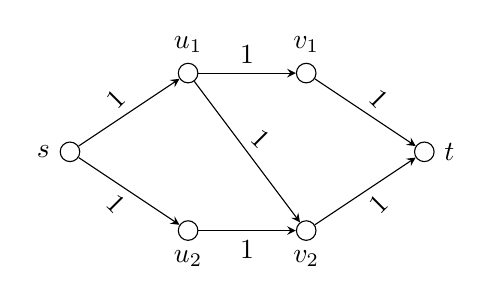
\begin{tikzpicture}
                \node[circle, draw, inner sep=2.5pt, label={180:$s$}] (s) at (-1.5, -1) {};
                \node[circle, draw, inner sep=2.5pt, label={90:$u_1$}] (u1) at (0, 0) {};
                \node[circle, draw, inner sep=2.5pt, label={90:$v_1$}] (v1) at (1.5, 0) {};
                \node[circle, draw, inner sep=2.5pt, label={-90:$u_2$}] (u2) at (0, -2) {};
                \node[circle, draw, inner sep=2.5pt, label={-90:$v_2$}] (v2) at (1.5, -2) {};
                \node[circle, draw, inner sep=2.5pt, label={0:$t$}] (t) at (3, -1) {};

                \draw[-stealth] (s) -- node[above, rotate=45] {1} (u1);
                \draw[-stealth] (s) -- node[below, rotate=-45] {1} (u2);
                \draw[-stealth] (u1) -- node[above] {1} (v1);
                \draw[-stealth] (u1) -- node[above, rotate=-45] {1} (v2);
                \draw[-stealth] (u2) -- node[below] {1} (v2);
                \draw[-stealth] (v1) -- node[above, rotate=-45] {1} (t);
                \draw[-stealth] (v2) -- node[below, rotate=45] {1} (t);
            \end{tikzpicture}
        \end{subfigure}
    \end{figure}
    \noindent On the left, we have an instance of maximum cardinality matching. Its equivalent instance is given on the right- the directed version of the edges present, along with the source $s$ and the sink $t$. Using the network flow algorithm, we will get the the same result. We illustrate this for the example above below:
    \begin{figure}[H]
        \centering
        \begin{subfigure}{0.45\textwidth}
            \centering
            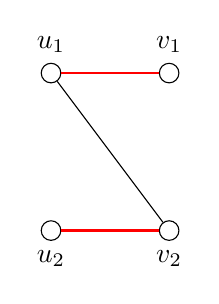
\begin{tikzpicture}
                \node[circle, draw, inner sep=2.5pt, label={90:$u_1$}] (u1) at (0, 0) {};
                \node[circle, draw, inner sep=2.5pt, label={90:$v_1$}] (v1) at (1.5, 0) {};
                \node[circle, draw, inner sep=2.5pt, label={-90:$u_2$}] (u2) at (0, -2) {};
                \node[circle, draw, inner sep=2.5pt, label={-90:$v_2$}] (v2) at (1.5, -2) {};

                \draw[red, thick] (u1) -- (v1);
                \draw (u1) -- (v2);
                \draw[red, thick] (u2) -- (v2);
            \end{tikzpicture}
        \end{subfigure}
        \hfill
        \begin{subfigure}{0.45\textwidth}
            \centering
            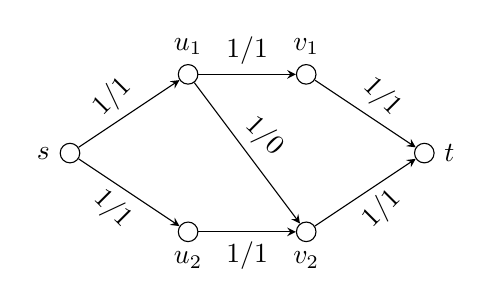
\begin{tikzpicture}
                \node[circle, draw, inner sep=2.5pt, label={180:$s$}] (s) at (-1.5, -1) {};
                \node[circle, draw, inner sep=2.5pt, label={90:$u_1$}] (u1) at (0, 0) {};
                \node[circle, draw, inner sep=2.5pt, label={90:$v_1$}] (v1) at (1.5, 0) {};
                \node[circle, draw, inner sep=2.5pt, label={-90:$u_2$}] (u2) at (0, -2) {};
                \node[circle, draw, inner sep=2.5pt, label={-90:$v_2$}] (v2) at (1.5, -2) {};
                \node[circle, draw, inner sep=2.5pt, label={0:$t$}] (t) at (3, -1) {};

                \draw[-stealth] (s) -- node[above, rotate=45] {1/1} (u1);
                \draw[-stealth] (s) -- node[below, rotate=-45] {1/1} (u2);
                \draw[-stealth] (u1) -- node[above] {1/1} (v1);
                \draw[-stealth] (u1) -- node[above, rotate=-45] {1/0} (v2);
                \draw[-stealth] (u2) -- node[below] {1/1} (v2);
                \draw[-stealth] (v1) -- node[above, rotate=-45] {1/1} (t);
                \draw[-stealth] (v2) -- node[below, rotate=45] {1/1} (t);
            \end{tikzpicture}
        \end{subfigure}
    \end{figure}
    \noindent The edges $\{u_1, v_1\}$ and $\{u_2, v_2\}$ are part of the maximum cardinality matching, as seen on the left. This can be inferred from right too- these edges are precisely those with flow value 1. If we use the network flow version of the algorithm, we will get a more efficient algorithm- it is $O(\sqrt{|V|}(|V| + |E|))$ instead of $O(|V| (|V| + |E|))$ we saw above.
    \newpage

    \section{Stable Marriage Problem}
    In this section, we discuss a matching problem called the Stable Marriage Problem. We are given the same number of students and lecturers, with preferences from both sides on who they would like to supervise/be supervised by, and we want to find an optimal matching. The optimal matching satisfies the condition that, if the lecturer/student were to be assigned to a different partner, then at least one of them would not be happy with it.

    We will consider optimality formally now. So, assume that we have 4 students and 4 lecturers, with the following preferences:
    \begin{table}[H]
        \centering
        \begin{subtable}{0.45\textwidth}
            \centering
            \begin{tabular}{c|cccc}
                $\texttt{s}_1$ & $\texttt{l}_2$ & $\texttt{l}_4$ & $\texttt{l}_1$ & $\texttt{l}_3$ \\
                $\texttt{s}_2$ & $\texttt{l}_3$ & $\texttt{l}_1$ & $\texttt{l}_4$ & $\texttt{l}_2$ \\
                $\texttt{s}_3$ & $\texttt{l}_2$ & $\texttt{l}_3$ & $\texttt{l}_1$ & $\texttt{l}_4$ \\
                $\texttt{s}_4$ & $\texttt{l}_4$ & $\texttt{l}_1$ & $\texttt{l}_3$ & $\texttt{l}_2$
            \end{tabular}
            \caption{Student's Preferences}
        \end{subtable}
        \hfill
        \begin{subtable}{0.45\textwidth}
            \centering
            \begin{tabular}{c|cccc}
                $\texttt{l}_1$ & $\texttt{s}_2$ & $\texttt{s}_1$ & $\texttt{s}_4$ & $\texttt{s}_3$ \\
                $\texttt{l}_2$ & $\texttt{s}_4$ & $\texttt{s}_3$ & $\texttt{s}_1$ & $\texttt{s}_2$ \\
                $\texttt{l}_3$ & $\texttt{s}_1$ & $\texttt{s}_4$ & $\texttt{s}_3$ & $\texttt{s}_2$ \\
                $\texttt{l}_4$ & $\texttt{s}_2$ & $\texttt{s}_1$ & $\texttt{s}_4$ & $\texttt{s}_3$
            \end{tabular}
            \caption{Lecturer's Preferences}
        \end{subtable}
    \end{table}
    \noindent One possible matching is the one given below:
    \begin{table}[H]
        \centering
        \begin{subtable}{0.45\textwidth}
            \centering
            \begin{tabular}{c|cccc}
                $\texttt{s}_1$ & $\texttt{l}_2$ & {\color{red} $\texttt{l}_4$} & \underline{$\texttt{l}_1$} & $\texttt{l}_3$ \\
                $\texttt{s}_2$ & \underline{$\texttt{l}_3$} & $\texttt{l}_1$ & $\texttt{l}_4$ & $\texttt{l}_2$ \\
                $\texttt{s}_3$ & \underline{$\texttt{l}_2$} & $\texttt{l}_3$ & $\texttt{l}_1$ & $\texttt{l}_4$ \\
                $\texttt{s}_4$ & \underline{$\texttt{l}_4$} & $\texttt{l}_1$ & $\texttt{l}_3$ & $\texttt{l}_2$
            \end{tabular}
        \end{subtable}
        \hfill
        \begin{subtable}{0.45\textwidth}
            \centering
            \begin{tabular}{c|cccc}
                $\texttt{l}_1$ & $\texttt{s}_2$ & \underline{$\texttt{s}_1$} & $\texttt{s}_4$ & $\texttt{s}_3$ \\
                $\texttt{l}_2$ & $\texttt{s}_4$ & \underline{$\texttt{s}_3$} & $\texttt{s}_1$ & $\texttt{s}_2$ \\
                $\texttt{l}_3$ & $\texttt{s}_1$ & $\texttt{s}_4$ & $\texttt{s}_3$ & \underline{$\texttt{s}_2$} \\
                $\texttt{l}_4$ & $\texttt{s}_2$ & {\color{red} $\texttt{s}_1$} & \underline{$\texttt{s}_4$} & $\texttt{s}_3$
            \end{tabular}
        \end{subtable}
    \end{table}
    \noindent So, we have the following pairs: $(\texttt{s}_1, \texttt{l}_1), (\texttt{s}_2, \texttt{l}_3), (\texttt{s}_3, \texttt{l}_2), (\texttt{s}_4, \texttt{l}_4)$ . This is not an optimal matching- $(\texttt{s}_1, \texttt{l}_4)$ is a matching where both the student and the lecturer prefer each other over the current matching. This is called a \emph{blocking pair}. The following is an optimal (stable) matching:
    \begin{table}[H]
        \centering
        \begin{subtable}{0.45\textwidth}
            \centering
            \begin{tabular}{c|cccc}
                $\texttt{s}_1$ & $\texttt{l}_2$ & \underline{$\texttt{l}_4$} & $\texttt{l}_1$ & $\texttt{l}_3$ \\
                $\texttt{s}_2$ & \underline{$\texttt{l}_3$} & $\texttt{l}_1$ & $\texttt{l}_4$ & $\texttt{l}_2$ \\
                $\texttt{s}_3$ & \underline{$\texttt{l}_2$} & $\texttt{l}_3$ & $\texttt{l}_1$ & $\texttt{l}_4$ \\
                $\texttt{s}_4$ & $\texttt{l}_4$ & \underline{$\texttt{l}_1$} & $\texttt{l}_3$ & $\texttt{l}_2$
            \end{tabular}
        \end{subtable}
        \hfill
        \begin{subtable}{0.45\textwidth}
            \centering
            \begin{tabular}{c|cccc}
                $\texttt{l}_1$ & $\texttt{s}_2$ & $\texttt{s}_1$ & \underline{$\texttt{s}_4$} & $\texttt{s}_3$ \\
                $\texttt{l}_2$ & $\texttt{s}_4$ & \underline{$\texttt{s}_3$} & $\texttt{s}_1$ & $\texttt{s}_2$ \\
                $\texttt{l}_3$ & $\texttt{s}_1$ & $\texttt{s}_4$ & $\texttt{s}_3$ & \underline{$\texttt{s}_2$} \\
                $\texttt{l}_4$ & $\texttt{s}_2$ & \underline{$\texttt{s}_1$} & $\texttt{s}_4$ & $\texttt{s}_3$
            \end{tabular}
        \end{subtable}
    \end{table}
    \noindent We will now show that it is a stable matching and has no blocking pairs. Clearly, $\texttt{s}_2$ and $\texttt{s}_3$ have their first choice, so they cannot lead to a blocking pair. Although $\texttt{s}_1$ would prefer $\texttt{l}_2$ over $\texttt{l}_4$, the lecturer $\texttt{l}_2$ prefers $\texttt{s}_3$ over $\texttt{s}_1$. The same is the case for $\texttt{s}_4$, which means that no student is part of a blocking pair, and hence there are no blocking pairs. So, this is a stable matching.

    Given a matching, we can check whether it is stable by checking whether any student is part of a blocking pair. That is, we iterate through all the students and check whether any lecturer they prefer to the one they are currently assigned would also prefer the student over their current assignee. We can do this in $O(n^2)$ time- in the worst case, the student has been assigned their last choice, so we have to look through almost all the lecturers, so the loop is $O(n^2)$. The body of the loop can be $O(1)$- we can make use of an efficient data structure to check whether a lecturer prefers a student over another one in constant time.

    We will now consider an algorithm to find the stable matching- the Gale-Shapley Algorithm. The following is the algorithm:
\begin{lstlisting}[language=pseudocode]
List<(Student, Lecturer)> galeShapley(List<Student> students, 
    List<Lecturer> lecturers) {
    Stack<Student> unmatched = students.toStack();
    List<(Student, Lecturer)> matches = [];
    while (unmatched.isNotEmpty) {
        Student s = unmatched.pop();
        Lecturer l = lecturers[s.currentChoice];
        if (l.isUnmatched) {
            matches.add(s, l);
        } else if (l.prefers(s, students[l.currentChoice])) {
            Student prevS = students[l.currentChoice];
            prevS.currentChoice = prevS.nextChoice;
            unmatched.push(prevS);
            matches.add(s, l);
        } else {
            s.currentChoice = s.nextChoice;
            unmatched.push(s);
        }
    }
    return matches;
}
\end{lstlisting}
    \noindent This is the student-oriented version of the algorithm- we are going down the student's preferences and finding the best lecturer for them. The algorithm runs until every student has been matched. Within the loop, we try to assign the student to some lecturer. We select the first lecturer that the student hasn't applied to- this is their \texttt{currentChoice}. If this lecturer is unassigned, we can provisionally match them. Otherwise, lecturer has two students that have applied to work with them- the lecturer rejects the one it prefers less, and this student is added back to the queue, where they will try the next choice. 
    
    We will now illustrate the algorithm. So, assume that we are starting with the following instance of the Stable Marriage Problem.
    \begin{table}[H]
        \centering
        \begin{subtable}{0.45\textwidth}
            \centering
            \begin{tabular}{c|cccc}
                $\texttt{s}_1$ & $\texttt{l}_2$ & $\texttt{l}_4$ & $\texttt{l}_1$ & $\texttt{l}_3$ \\
                $\texttt{s}_2$ & $\texttt{l}_3$ & $\texttt{l}_1$ & $\texttt{l}_4$ & $\texttt{l}_2$ \\
                $\texttt{s}_3$ & $\texttt{l}_2$ & $\texttt{l}_3$ & $\texttt{l}_1$ & $\texttt{l}_4$ \\
                $\texttt{s}_4$ & $\texttt{l}_4$ & $\texttt{l}_1$ & $\texttt{l}_3$ & $\texttt{l}_2$
            \end{tabular}
            \caption{Student's Preferences}
        \end{subtable}
        \hfill
        \begin{subtable}{0.45\textwidth}
            \centering
            \begin{tabular}{c|cccc}
                $\texttt{l}_1$ & $\texttt{s}_2$ & $\texttt{s}_1$ & $\texttt{s}_4$ & $\texttt{s}_3$ \\
                $\texttt{l}_2$ & $\texttt{s}_4$ & $\texttt{s}_3$ & $\texttt{s}_1$ & $\texttt{s}_2$ \\
                $\texttt{l}_3$ & $\texttt{s}_1$ & $\texttt{s}_4$ & $\texttt{s}_3$ & $\texttt{s}_2$ \\
                $\texttt{l}_4$ & $\texttt{s}_2$ & $\texttt{s}_1$ & $\texttt{s}_4$ & $\texttt{s}_3$
            \end{tabular}
            \caption{Lecturer's Preferences}
        \end{subtable}
    \end{table}
    \noindent We will match the students to the lecturers, going from their top preference to the last. 
    \begin{table}[H]
        \centering
        \begin{subtable}{0.45\textwidth}
            \centering
            \begin{tabular}{c|cccc}
                $\texttt{s}_1$ & \underline{$\texttt{l}_2$} & $\texttt{l}_4$ & $\texttt{l}_1$ & $\texttt{l}_3$ \\
                $\texttt{s}_2$ & $\texttt{l}_3$ & $\texttt{l}_1$ & $\texttt{l}_4$ & $\texttt{l}_2$ \\
                $\texttt{s}_3$ & $\texttt{l}_2$ & $\texttt{l}_3$ & $\texttt{l}_1$ & $\texttt{l}_4$ \\
                $\texttt{s}_4$ & $\texttt{l}_4$ & $\texttt{l}_1$ & $\texttt{l}_3$ & $\texttt{l}_2$
            \end{tabular}
        \end{subtable}
        \hfill
        \begin{subtable}{0.45\textwidth}
            \centering
            \begin{tabular}{c|cccc}
                $\texttt{l}_1$ & $\texttt{s}_2$ & $\texttt{s}_1$ & $\texttt{s}_4$ & $\texttt{s}_3$ \\
                $\texttt{l}_2$ & $\texttt{s}_4$ & $\texttt{s}_3$ & \underline{$\texttt{s}_1$} & $\texttt{s}_2$ \\
                $\texttt{l}_3$ & $\texttt{s}_1$ & $\texttt{s}_4$ & $\texttt{s}_3$ & $\texttt{s}_2$ \\
                $\texttt{l}_4$ & $\texttt{s}_2$ & $\texttt{s}_1$ & $\texttt{s}_4$ & $\texttt{s}_3$
            \end{tabular}
        \end{subtable}
    \end{table}
    \noindent So, we start with matching $(\texttt{s}_1, \texttt{l}_2)$. It might end up being changed, but they are paired at this point. 
    \begin{table}[H]
        \centering
        \begin{subtable}{0.45\textwidth}
            \centering
            \begin{tabular}{c|cccc}
                $\texttt{s}_1$ & \underline{$\texttt{l}_2$} & $\texttt{l}_4$ & $\texttt{l}_1$ & $\texttt{l}_3$ \\
                $\texttt{s}_2$ & \underline{$\texttt{l}_3$} & $\texttt{l}_1$ & $\texttt{l}_4$ & $\texttt{l}_2$ \\
                $\texttt{s}_3$ & $\texttt{l}_2$ & $\texttt{l}_3$ & $\texttt{l}_1$ & $\texttt{l}_4$ \\
                $\texttt{s}_4$ & $\texttt{l}_4$ & $\texttt{l}_1$ & $\texttt{l}_3$ & $\texttt{l}_2$
            \end{tabular}
        \end{subtable}
        \hfill
        \begin{subtable}{0.45\textwidth}
            \centering
            \begin{tabular}{c|cccc}
                $\texttt{l}_1$ & $\texttt{s}_2$ & $\texttt{s}_1$ & $\texttt{s}_4$ & $\texttt{s}_3$ \\
                $\texttt{l}_2$ & $\texttt{s}_4$ & $\texttt{s}_3$ & \underline{$\texttt{s}_1$} & $\texttt{s}_2$ \\
                $\texttt{l}_3$ & $\texttt{s}_1$ & $\texttt{s}_4$ & $\texttt{s}_3$ & \underline{$\texttt{s}_2$} \\
                $\texttt{l}_4$ & $\texttt{s}_2$ & $\texttt{s}_1$ & $\texttt{s}_4$ & $\texttt{s}_3$
            \end{tabular}
        \end{subtable}
    \end{table}
    \noindent Similarly, we can match $(\texttt{s}_2, \texttt{l}_3)$. This is still a valid matching.
    \begin{table}[H]
        \centering
        \begin{subtable}{0.45\textwidth}
            \centering
            \begin{tabular}{c|cccc}
                $\texttt{s}_1$ & \underline{$\texttt{l}_2$} & $\texttt{l}_4$ & $\texttt{l}_1$ & $\texttt{l}_3$ \\
                $\texttt{s}_2$ & \underline{$\texttt{l}_3$} & $\texttt{l}_1$ & $\texttt{l}_4$ & $\texttt{l}_2$ \\
                $\texttt{s}_3$ & \underline{$\texttt{l}_2$} & $\texttt{l}_3$ & $\texttt{l}_1$ & $\texttt{l}_4$ \\
                $\texttt{s}_4$ & $\texttt{l}_4$ & $\texttt{l}_1$ & $\texttt{l}_3$ & $\texttt{l}_2$
            \end{tabular}
        \end{subtable}
        \hfill
        \begin{subtable}{0.45\textwidth}
            \centering
            \begin{tabular}{c|cccc}
                $\texttt{l}_1$ & $\texttt{s}_2$ & $\texttt{s}_1$ & $\texttt{s}_4$ & $\texttt{s}_3$ \\
                $\texttt{l}_2$ & $\texttt{s}_4$ & \underline{$\texttt{s}_3$} & \underline{$\texttt{s}_1$} & $\texttt{s}_2$ \\
                $\texttt{l}_3$ & $\texttt{s}_1$ & $\texttt{s}_4$ & $\texttt{s}_3$ & \underline{$\texttt{s}_2$} \\
                $\texttt{l}_4$ & $\texttt{s}_2$ & $\texttt{s}_1$ & $\texttt{s}_4$ & $\texttt{s}_3$
            \end{tabular}
        \end{subtable}
    \end{table}
    \noindent Next, we try to match $\texttt{s}_3$. Their first choice is $\texttt{l}_2$, but they are currently paired with $\texttt{s}_1$. The lecturer $\texttt{l}_2$ prefers $\texttt{s}_3$ over $\texttt{s}_1$, so $\texttt{l}_2$ rejects $\texttt{s}_1$. 
    \begin{table}[H]
        \centering
        \begin{subtable}{0.45\textwidth}
            \centering
            \begin{tabular}{c|cccc}
                $\texttt{s}_1$ & {\color{blue!60} $\texttt{l}_2$} & $\texttt{l}_4$ & $\texttt{l}_1$ & $\texttt{l}_3$ \\
                $\texttt{s}_2$ & \underline{$\texttt{l}_3$} & $\texttt{l}_1$ & $\texttt{l}_4$ & $\texttt{l}_2$ \\
                $\texttt{s}_3$ & \underline{$\texttt{l}_2$} & $\texttt{l}_3$ & $\texttt{l}_1$ & $\texttt{l}_4$ \\
                $\texttt{s}_4$ & $\texttt{l}_4$ & $\texttt{l}_1$ & $\texttt{l}_3$ & $\texttt{l}_2$
            \end{tabular}
        \end{subtable}
        \hfill
        \begin{subtable}{0.45\textwidth}
            \centering
            \begin{tabular}{c|cccc}
                $\texttt{l}_1$ & $\texttt{s}_2$ & $\texttt{s}_1$ & $\texttt{s}_4$ & $\texttt{s}_3$ \\
                $\texttt{l}_2$ & $\texttt{s}_4$ & \underline{$\texttt{s}_3$} & $\texttt{s}_1$ & $\texttt{s}_2$ \\
                $\texttt{l}_3$ & $\texttt{s}_1$ & $\texttt{s}_4$ & $\texttt{s}_3$ & \underline{$\texttt{s}_2$} \\
                $\texttt{l}_4$ & $\texttt{s}_2$ & $\texttt{s}_1$ & $\texttt{s}_4$ & $\texttt{s}_3$
            \end{tabular}
        \end{subtable}
    \end{table}
    \noindent Hence, $\texttt{s}_1$ is unmatched, so we try to match it with its next choice- $\texttt{l}_4$.
    \begin{table}[H]
        \centering
        \begin{subtable}{0.45\textwidth}
            \centering
            \begin{tabular}{c|cccc}
                $\texttt{s}_1$ & {\color{blue!60} $\texttt{l}_2$} & \underline{$\texttt{l}_4$} & $\texttt{l}_1$ & $\texttt{l}_3$ \\
                $\texttt{s}_2$ & \underline{$\texttt{l}_3$} & $\texttt{l}_1$ & $\texttt{l}_4$ & $\texttt{l}_2$ \\
                $\texttt{s}_3$ & \underline{$\texttt{l}_2$} & $\texttt{l}_3$ & $\texttt{l}_1$ & $\texttt{l}_4$ \\
                $\texttt{s}_4$ & $\texttt{l}_4$ & $\texttt{l}_1$ & $\texttt{l}_3$ & $\texttt{l}_2$
            \end{tabular}
        \end{subtable}
        \hfill
        \begin{subtable}{0.45\textwidth}
            \centering
            \begin{tabular}{c|cccc}
                $\texttt{l}_1$ & $\texttt{s}_2$ & $\texttt{s}_1$ & $\texttt{s}_4$ & $\texttt{s}_3$ \\
                $\texttt{l}_2$ & $\texttt{s}_4$ & \underline{$\texttt{s}_3$} & $\texttt{s}_1$ & $\texttt{s}_2$ \\
                $\texttt{l}_3$ & $\texttt{s}_1$ & $\texttt{s}_4$ & $\texttt{s}_3$ & \underline{$\texttt{s}_2$} \\
                $\texttt{l}_4$ & $\texttt{s}_2$ & \underline{$\texttt{s}_1$} & $\texttt{s}_4$ & $\texttt{s}_3$
            \end{tabular}
        \end{subtable}
    \end{table}
    \noindent The pair $(\texttt{s}_1, \texttt{l}_4)$ is a valid match for now.
    \begin{table}[H]
        \centering
        \begin{subtable}{0.45\textwidth}
            \centering
            \begin{tabular}{c|cccc}
                $\texttt{s}_1$ & {\color{blue!60} $\texttt{l}_2$} & \underline{$\texttt{l}_4$} & $\texttt{l}_1$ & $\texttt{l}_3$ \\
                $\texttt{s}_2$ & \underline{$\texttt{l}_3$} & $\texttt{l}_1$ & $\texttt{l}_4$ & $\texttt{l}_2$ \\
                $\texttt{s}_3$ & \underline{$\texttt{l}_2$} & $\texttt{l}_3$ & $\texttt{l}_1$ & $\texttt{l}_4$ \\
                $\texttt{s}_4$ & \underline{$\texttt{l}_4$} & $\texttt{l}_1$ & $\texttt{l}_3$ & $\texttt{l}_2$
            \end{tabular}
        \end{subtable}
        \hfill
        \begin{subtable}{0.45\textwidth}
            \centering
            \begin{tabular}{c|cccc}
                $\texttt{l}_1$ & $\texttt{s}_2$ & $\texttt{s}_1$ & $\texttt{s}_4$ & $\texttt{s}_3$ \\
                $\texttt{l}_2$ & $\texttt{s}_4$ & \underline{$\texttt{s}_3$} & $\texttt{s}_1$ & $\texttt{s}_2$ \\
                $\texttt{l}_3$ & $\texttt{s}_1$ & $\texttt{s}_4$ & $\texttt{s}_3$ & \underline{$\texttt{s}_2$} \\
                $\texttt{l}_4$ & $\texttt{s}_2$ & \underline{$\texttt{s}_1$} & \underline{$\texttt{s}_4$} & $\texttt{s}_3$
            \end{tabular}
        \end{subtable}
    \end{table}
    \noindent Next, we match $\texttt{s}_4$ with $\texttt{l}_4$. The lecturer $\texttt{l}_4$ now has two offers- from $\texttt{s}_1$ and $\texttt{s}_4$, and they prefer $\texttt{s}_1$ over $\texttt{s}_4$. 
    \begin{table}[H]
        \centering
        \begin{subtable}{0.45\textwidth}
            \centering
            \begin{tabular}{c|cccc}
                $\texttt{s}_1$ & {\color{blue!60} $\texttt{l}_2$} & \underline{$\texttt{l}_4$} & $\texttt{l}_1$ & $\texttt{l}_3$ \\
                $\texttt{s}_2$ & \underline{$\texttt{l}_3$} & $\texttt{l}_1$ & $\texttt{l}_4$ & $\texttt{l}_2$ \\
                $\texttt{s}_3$ & \underline{$\texttt{l}_2$} & $\texttt{l}_3$ & $\texttt{l}_1$ & $\texttt{l}_4$ \\
                $\texttt{s}_4$ & {\color{blue!60} $\texttt{l}_4$} & $\texttt{l}_1$ & $\texttt{l}_3$ & $\texttt{l}_2$
            \end{tabular}
        \end{subtable}
        \hfill
        \begin{subtable}{0.45\textwidth}
            \centering
            \begin{tabular}{c|cccc}
                $\texttt{l}_1$ & $\texttt{s}_2$ & $\texttt{s}_1$ & $\texttt{s}_4$ & $\texttt{s}_3$ \\
                $\texttt{l}_2$ & $\texttt{s}_4$ & \underline{$\texttt{s}_3$} & $\texttt{s}_1$ & $\texttt{s}_2$ \\
                $\texttt{l}_3$ & $\texttt{s}_1$ & $\texttt{s}_4$ & $\texttt{s}_3$ & \underline{$\texttt{s}_2$} \\
                $\texttt{l}_4$ & $\texttt{s}_2$ & \underline{$\texttt{s}_1$} & $\texttt{s}_4$ & $\texttt{s}_3$
            \end{tabular}
        \end{subtable}
    \end{table}
    \noindent So, $\texttt{s}_4$ gets rejected by $\texttt{l}_4$.
    \begin{table}[H]
        \centering
        \begin{subtable}{0.45\textwidth}
            \centering
            \begin{tabular}{c|cccc}
                $\texttt{s}_1$ & {\color{blue!60} $\texttt{l}_2$} & \underline{$\texttt{l}_4$} & $\texttt{l}_1$ & $\texttt{l}_3$ \\
                $\texttt{s}_2$ & \underline{$\texttt{l}_3$} & $\texttt{l}_1$ & $\texttt{l}_4$ & $\texttt{l}_2$ \\
                $\texttt{s}_3$ & \underline{$\texttt{l}_2$} & $\texttt{l}_3$ & $\texttt{l}_1$ & $\texttt{l}_4$ \\
                $\texttt{s}_4$ & {\color{blue!60}$\texttt{l}_4$} & \underline{$\texttt{l}_1$} & $\texttt{l}_3$ & $\texttt{l}_2$
            \end{tabular}
        \end{subtable}
        \hfill
        \begin{subtable}{0.45\textwidth}
            \centering
            \begin{tabular}{c|cccc}
                $\texttt{l}_1$ & $\texttt{s}_2$ & $\texttt{s}_1$ & \underline{$\texttt{s}_4$} & $\texttt{s}_3$ \\
                $\texttt{l}_2$ & $\texttt{s}_4$ & \underline{$\texttt{s}_3$} & $\texttt{s}_1$ & $\texttt{s}_2$ \\
                $\texttt{l}_3$ & $\texttt{s}_1$ & $\texttt{s}_4$ & $\texttt{s}_3$ & \underline{$\texttt{s}_2$} \\
                $\texttt{s}_4$ & $\texttt{s}_2$ & \underline{$\texttt{s}_1$} & $\texttt{s}_4$ & $\texttt{s}_3$
            \end{tabular}
        \end{subtable}
    \end{table}
    \noindent Next, we match $\texttt{s}_4$ with $\texttt{l}_1$. The lecturer $\texttt{l}_1$ wasn't assigned before, so $(\texttt{l}_1, \texttt{s}_4)$ gives the final matching. All the students have been matched, so the algorithm terminates- we have found a stable matching.

    We will now show that the Gale-Shapley algorithm terminates with every student assigned. In particular, we claim that no student gets rejected by all the lecturers. Assume, for a contradiction, that the student $s$ gets rejected by all the lecturers. This can only happen if all the lecturers have been assigned to a student at that point during the algorithm. However, if a lecturer is assigned at some point, they remain assigned (they might change who they are matched to, but they do not become unmatched). This implies that when $s$ was rejected by the last lecturer in its preference list, all the lecturers were assigned. However, there are the same number of students and lecturers, and a student cannot be assigned to more than one lecturer. This is a contradiction- no student can be rejected by all the lecturers. Hence, every student gets accepted by some lecturer, meaning that the algorithm terminates. 
    
    Next, we show that the algorithm terminates with the stable matching. When the algorithm terminates, we have a matching containing all the students. Let $s$ be a student and let $l$ be a lecturer that $s$ prefers over its matching. This means that, at some point during the algorithm, $s$ applied to $l$. Moreover, since $(s, l)$ is not in the matching, we know that $l$ rejected $s$ at some point. The only reason this could happen is if $l$ got an offer from a student that they preferred over $s$. Hence, $(s, l)$ cannot be a blocking pair. So, there is no blocking pair in the matching- it is stable. This also shows that every instance of the Stable Marriage Problem has a stable matching.
    
    We now consider the complexity of the algorithm. In the worst case, a student might only be accepted by the last lecturer in its list, so the while loop can run $O(n^2)$ times. The body of the while loop is constant time (we can check whether a lecturer prefers a student over another in constant time). A student applies to a student just once, so the algorithm has $O(n^2)$ time complexity. Note that the algorithm is linear in size of the input- the input is the preference list which has $O(n^2)$ space complexity for both students and lecturers.

    The Gale-Shapley algorithm given above is non-deterministic- the order in which the students apply to the lecturers is not specified. But, it turns out that this does not affect the final outcome of the algorithm- every ordering in which the students apply will give the same result. Moreover, in the student-oriented Gale-Shapley algorithm, every student gets their best lecturer choice, while every lecturer gets their worst student choice.

    We shall now consider how to implement the algorithm in $O(n^2)$ time. In particular, we will show how to compute whether a lecturer prefers a student over another in $O(1)$ time. To do so, we assume that the preferences are given as two matrices (lists of lists)- \texttt{sp} for student preferences and \texttt{lp} for lecturer preferences, e.g. \texttt{sp[s, i] = l} if \texttt{s} has the lecturer \texttt{l} at \texttt{i}-th position in their preference list. Using these matrices, we construct the lecturer's ranking lists- \texttt{lr[l, s] = i} if \texttt{lp[l, i] = s}. For instance, assume that the \texttt{lp} matrix is the following:
    \[\texttt{lp} = \begin{bmatrix}
        \texttt{s}_2 & \texttt{s}_1 & \texttt{s}_4 & \texttt{s}_3 \\
        \texttt{s}_4 & \texttt{s}_3 & \texttt{s}_1 & \texttt{s}_2 \\
        \texttt{s}_1 & \texttt{s}_4 & \texttt{s}_3 & \texttt{s}_2 \\
        \texttt{s}_2 & \texttt{s}_1 & \texttt{s}_4 & \texttt{s}_3
    \end{bmatrix}.\]
    So, we have $\texttt{lp}[\texttt{l}_1, 0] = \texttt{s}_2$. Then, the \texttt{lr} matrix is the following:
    \[\texttt{lr} = \begin{bmatrix}
        1 & 0 & 3 & 2 \\
        2 & 3 & 1 & 0 \\
        0 & 3 & 2 & 1 \\
        1 & 0 & 3 & 2
    \end{bmatrix}.\]
    From this matrix, we can tell whether a lecturer prefers a student over another in constant time. For instance, $\texttt{l}_1$ prefers $\texttt{s}_2$ over $\texttt{s}_1$ since $\texttt{lr}[\texttt{l}_1, \texttt{s}_2] = 0 < 1 = \texttt{lr}[\texttt{l}_1, \texttt{s}_1]$. We can construct the ranking table for all the lecturers at the start of the algorithm in $O(n^2)$ time.

    \newpage

    \section{All Pairs Shortest Paths}
    In this section, we will look at an algorithm to find all pairs of shortest paths in a weighted directed graph. That is, for a pair $(v, w)$ of vertices in the graph, we want to find a path from $v$ to $w$ which has the smallest weight. We will allow the weights in the graph to be negative, and will consider how to deal with this complication as well.

    Assume that we have the following weighted directed graph.
    \begin{figure}[H]
        \centering
        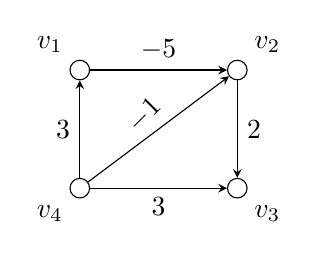
\begin{tikzpicture}
            \node[inner sep=2.5pt, draw, circle, label={135:$v_1$}] (1) at (0, 0) {};
            \node[inner sep=2.5pt, draw, circle, label={45:$v_2$}] (2) at (2, 0) {};
            \node[inner sep=2.5pt, draw, circle, label={-45:$v_3$}] (3) at (2, -1.5) {};
            \node[inner sep=2.5pt, draw, circle, label={-135:$v_4$}] (4) at (0, -1.5) {};
            
            \draw[-stealth] (1) -- node[above] {$-5$} (2);
            \draw[-stealth] (2) -- node[right] {$2$} (3);
            \draw[-stealth] (4) -- node[left] {$3$} (1);
            \draw[-stealth] (4) -- node[above, rotate=45] {$-1$} (2);
            \draw[-stealth] (4) -- node[below] {$3$} (3);
        \end{tikzpicture}
    \end{figure}
    \noindent The following matrix gives the weight of the shortest path between any pair of vertices.
    \[D^* = \begin{bmatrix}
        0 & -5 & -3 & \infty \\
        \infty & 0 & 2 & \infty \\
        \infty & \infty & 0 & \infty \\
        3 & -2 & 0  & 0
    \end{bmatrix}\]
    Every diagonal entry is 0- traveling from a vertex to itself should not cost anything\sidefootnote{And it also shouldn't be profitable!}. If a distance is $\infty$, then there is no path between the two vertices, e.g. there is no path from $v_1$ to $v_4$. Since we allow negative weights, it is possible that the shortest path between two vertices has negative value, e.g. the best path from $v_4$ to $v_2$ has weight $-2$- the path is $v_4 \to v_1 \to v_2$.

    We have previously seen the Dijkstra's algorithm to find the path of smallest weight from a vertex to all the other vertices. It takes $O(n^2)$ time (or $O(n \log n + m)$ using a Fibonacci heap), where $n = |V|$ and $m = |E|$. So, we could use this algorithm to get all pairs shortest paths in $O(n^3)$ time applying the algorithm to all the vertices. However, this algorithm does not work with edges that have negative weight. For instance, consider the following graph:
    \begin{figure}[H]
        \centering
        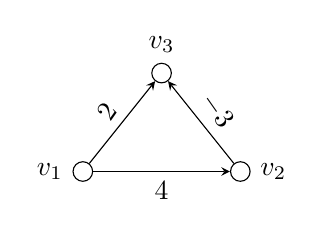
\begin{tikzpicture}
            \node[inner sep=2.5pt, draw, circle, label={180:$v_1$}] (1) at (0, 0) {};
            \node[inner sep=2.5pt, draw, circle, label={0:$v_2$}] (2) at (2, 0) {};
            \node[inner sep=2.5pt, draw, circle, label={90:$v_3$}] (3) at (1, 1.25) {};

            \draw[-stealth] (1) -- node[below] {4} (2);
            \draw[-stealth] (1) -- node[above, rotate=55] {2} (3);
            \draw[-stealth] (2) -- node[above, rotate=-55] {$-3$} (3);
        \end{tikzpicture}
    \end{figure}
    \noindent When computing the path of smallest weight from $v_1$, the algorithm iterates as follows:
    \begin{itemize}
        \item $v_1$ has an edge to $v_3$ of shortest weight, so $v_1 - v_3$ has weight 2;
        \item $v_3$ has an edge to $v_2$ of shortest weight, so $v_1 - v_2$ has weight $-1$.
    \end{itemize}
    However, it is possible to take the path $v_1 - v_2 - v_3$ to get a path of weight 1. We cannot find this since the algorithm is greedy.

    Alternatively, we can use the Bellman-Ford algorithm which can handle negative weights. It has complexity $O(mn)$. So, if we used this algorithm to find all pairs shortest paths, it would take $O(mn^2)$ time. If the graph is dense (i.e. a lot of edges), then this is $O(n^4)$. We will now look at the Floyd-Warshall algorithm which computes all pairs shortest paths in $O(n^3)$ time, using dynamic programming. Although the algorithm works with negative edge weights, it won't work for graphs with negative cycles. For instance, consider the following graph:
    \begin{figure}[H]
        \centering
        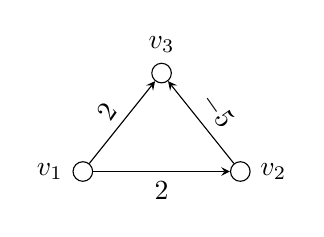
\begin{tikzpicture}
            \node[inner sep=2.5pt, draw, circle, label={180:$v_1$}] (1) at (0, 0) {};
            \node[inner sep=2.5pt, draw, circle, label={0:$v_2$}] (2) at (2, 0) {};
            \node[inner sep=2.5pt, draw, circle, label={90:$v_3$}] (3) at (1, 1.25) {};

            \draw[-stealth] (1) -- node[below] {2} (2);
            \draw[-stealth] (1) -- node[above, rotate=55] {2} (3);
            \draw[-stealth] (2) -- node[above, rotate=-55] {$-5$} (3);
        \end{tikzpicture}
    \end{figure}
    \noindent In this graph, the loop $v_1 - v_3 - v_2 - v_1$ has weight $-1$, which means that we can loop around the graph as many times as we wish to decrease the length of the shortest path for any two vertices. The Floyd-Warshall algorithm will give unexpected results when used on graphs with negative cycles.
    
    We will now consider how the Floyd-Warshall algorithm works. During the algorithm, we iterate $n$ times, and keep track of the current all-pair shortest path matrix. During an iteration $i$, we improve the weight of the shortest path by allowing vertex $v_i$ to be part of the shortest path. In particular, we compare whether the current shortest path from a vertex $v_a$ to another vertex $v_b$ with the current shortest path from vertex $v_a$ to $v_i$ and $v_i$ to $v_b$. If the latter is the smaller one, we update the value; otherwise, we keep it as is. We store these values in distance matrices $D_i$. So, the matrix $D_i$ stores the shortest path distance from any pair of vertices that goes through the vertices $v_1, v_2, \dots, v_i$. Hence, after the algorithm terminates, the distance matrix $D_n$ holds the values of all pairs shortest paths.

    Next, we will look at the dynamic programming algorithm formally. At the start, the matrix $D_0$ is given as follows:
    \[D_0[i, j] = \begin{cases}
        0 & i = j \\
        wt(v_i, v_j) & (v_i, v_j) \in E \\
        \infty & \text{otherwise}.
    \end{cases}\]
    The matrix $D_0$ represents the length of the (shortest) path going from a vertex to another that does not involve any other vertex. This equals the weight of the edge between the two vertices, if it exists. If the two vertices are the same, then the weight is 0 (assuming there are no negative cycles). If the two vertices are different and have no edge between them, then there is no path at this point- we denote this by $\infty$. Now, we construct the matrix $D_k$ from $D_{k-1}$ as follows:
    \[D_k[i, j] = \min (D_{k-1}[i, j], D_{k-1}[i, k] + D_{k-1}[k, j]).\]
    This follows from what we mentioned above- the distance from vertex $v_i$ to $v_j$ is either the previous distance, or the distance going through vertex $v_k$.

    We now consider the algorithm.
\begin{lstlisting}[language=pseudocode]
List<List<int>> floydWarshall(Graph graph) {
    List<List<int>> dPrev = List.filled(graph.vertices.length, 
        List(graph.vertices.length)
    );
    for (int i=0; i<graph.vertices.length; i++) {
        for (int j=0; j<graph.vertices.length; i++) {
            if (i == j) {
                dPrev[i, j] = 0;
            } else {
                dPrev[i, j] = graph.adjMatrix[i, j];
            }
        }
    }

    for (int k=1; k<graph.vertices.length; i++) {
        List<List<int>> dNext = List.filled(graph.vertices.length, 
            List(graph.vertices.length)
        );
        for (int i=0; i<graph.vertices.length; i++) {
            for (int j=0; j<graph.vertices.length; j++) {
                dNext[i, j] = min(dPrev[i, j],
                    dPrev[i, k] + dPrev[k, j]
                );
            }
        }
        dPrev = dNext;
    }
    return distanceMatrices[graph.vertices.length-1];
}
\end{lstlisting}
    From the algorithm, it is clear that the Floyd-Warshall has $O(n^3)$ time complexity and $O(n^2)$ space complexity.

    Using the Floyd-Warshall algorithm, we can detect whether a graph has negative cycle. In particular, if $D^*[i, i] \neq 0$ for any vertex $v_i$, the graph has a negative cycle.

    Along with the length of the shortest path between two vertices, we would also like to compute that path. To do so, it suffices to store the predecessor vertex in the path- we can follow the predecessor vertex until we get to the first vertex. So, we can also keep track of the predecessor vertices in the algorithm. These are stored in a dynamic programming matrix like with the distance matrix. In particular, 
    \[\Pi_0[i, j] = \begin{cases}
        \texttt{null} & i = j \\
        i & (v_i, v_j) \in E \\
        \texttt{null} & \text{otherwise},
    \end{cases} \quad \Pi_k[i, j] = \begin{cases}
        \Pi_{k-1}[i, j] & D_k[i, j] = D_{k-1}[i, j] \\
        \Pi_k[k, j] & \text{otherwise}.
    \end{cases}\]
    At the start, the only paths we have are of length 1, so the predecessor of a path from $v_i$ to $v_j$ is $v_i$. There is no predecessor for paths of length 0. In the recursive case, if we stick to the previous weight, then the predecessor vertex also remains the same. Otherwise, the shortest path from $v_i$ to $v_j$ is now $v_i - \dots - v_k - \dots - v_j$, meaning that the predecessor is the same as the one for the path $v_k - \dots - v_j$. The final predecessor matrix $\Pi_n$ gives the predecessor for the all pairs shortest path.

    We will now illustrate the algorithm with an example. So, assume that we have the following weighted directed graph.    
    \begin{figure}[H]
        \centering
        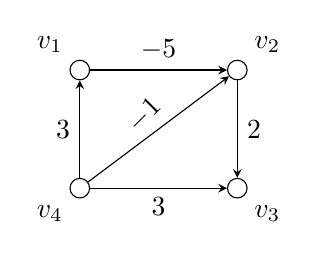
\begin{tikzpicture}
            \node[inner sep=2.5pt, draw, circle, label={135:$v_1$}] (1) at (0, 0) {};
            \node[inner sep=2.5pt, draw, circle, label={45:$v_2$}] (2) at (2, 0) {};
            \node[inner sep=2.5pt, draw, circle, label={-45:$v_3$}] (3) at (2, -1.5) {};
            \node[inner sep=2.5pt, draw, circle, label={-135:$v_4$}] (4) at (0, -1.5) {};
            
            \draw[-stealth] (1) -- node[above] {$-5$} (2);
            \draw[-stealth] (2) -- node[right] {$2$} (3);
            \draw[-stealth] (4) -- node[left] {$3$} (1);
            \draw[-stealth] (4) -- node[above, rotate=45] {$-1$} (2);
            \draw[-stealth] (4) -- node[below] {$3$} (3);
        \end{tikzpicture}
    \end{figure}
    \noindent Originally, we have the following initial distance matrix $D_0$ and initial predecessor matrix $\Pi_0$:
    \[D_0 = \begin{bmatrix}
        0 & -5 & \infty & \infty \\
        \infty & 0 & 2 & \infty \\
        \infty & \infty & 0 & \infty \\
        3 & -1 & 3 & 0
    \end{bmatrix}, \qquad \Pi_0 = \begin{bmatrix}
        \texttt{null} & 1 & \texttt{null} & \texttt{null} \\
        \texttt{null} & \texttt{null} & 2 & \texttt{null} \\
        \texttt{null} & \texttt{null} & \texttt{null} & \texttt{null} \\
        4 & 4 & 4 & \texttt{null}
    \end{bmatrix}.\]
    \noindent We will now construct $D_1$- this involves the vertex $v_1$.
    \begin{figure}[H]
        \centering
        \begin{tikzpicture}
            \node[fill=red, inner sep=2.5pt, draw, circle, label={135:$v_1$}] (1) at (0, 0) {};
            \node[inner sep=2.5pt, draw, circle, label={45:$v_2$}] (2) at (2, 0) {};
            \node[inner sep=2.5pt, draw, circle, label={-45:$v_3$}] (3) at (2, -1.5) {};
            \node[inner sep=2.5pt, draw, circle, label={-135:$v_4$}] (4) at (0, -1.5) {};
            
            \draw[-stealth, dashed] (1) -- node[above] {$-5$} (2);
            \draw[-stealth] (2) -- node[right] {$2$} (3);
            \draw[-stealth, dashed] (4) -- node[left] {$3$} (1);
            \draw[-stealth] (4) -- node[above, rotate=45] {$-1$} (2);
            \draw[-stealth] (4) -- node[below] {$3$} (3);
        \end{tikzpicture}
    \end{figure}
    \noindent So, the edges we have access to are $(v_4, v_1)$ and $(v_1, v_2)$. The only path we can improve is the one from $v_4$ to $v_2$- the current weight is $-1$, but we can make it $-2$ through this path.
    \[D_1 = \begin{bmatrix}
        0 & -5 & \infty & \infty \\
        \infty & 0 & 2 & \infty \\
        \infty & \infty & 0 & \infty \\
        3 & {\color{red} -2} & 3 & 0
    \end{bmatrix}, \qquad \Pi_1 = \begin{bmatrix}
        \texttt{null} & 1 & \texttt{null} & \texttt{null} \\
        \texttt{null} & \texttt{null} & 2 & \texttt{null} \\
        \texttt{null} & \texttt{null} & \texttt{null} & \texttt{null} \\
        4 & {\color{red} 1} & 4 & \texttt{null}
    \end{bmatrix}.\]
    \noindent Along with the distance, the predecessor value also changes- the predecessor edge in the path from $v_4$ to $v_2$ is now $v_1$, not $v_4$. We next allow edges going through the vertex $v_2$:
    \begin{figure}[H]
        \centering
        \begin{tikzpicture}
            \node[fill=red, inner sep=2.5pt, draw, circle, label={135:$v_1$}] (1) at (0, 0) {};
            \node[fill=red, inner sep=2.5pt, draw, circle, label={45:$v_2$}] (2) at (2, 0) {};
            \node[inner sep=2.5pt, draw, circle, label={-45:$v_3$}] (3) at (2, -1.5) {};
            \node[inner sep=2.5pt, draw, circle, label={-135:$v_4$}] (4) at (0, -1.5) {};
            
            \draw[-stealth, dotted] (1) -- node[above] {$-5$} (2);
            \draw[-stealth, dashed] (2) -- node[right] {$2$} (3);
            \draw[-stealth, dotted] (4) -- node[left] {$3$} (1);
            \draw[-stealth, dashed] (4) -- node[above, rotate=45] {$-1$} (2);
            \draw[-stealth] (4) -- node[below] {$3$} (3);
        \end{tikzpicture}
    \end{figure}
    \noindent So, the paths we can improve go from $v_1$ to $v_3$; from $v_4$ to $v_3$. In both cases, we can improve them from the current value- the current weight from $v_1$ to $v_3$ is $\infty$. 
    \[D_2 = \begin{bmatrix}
        0 & -5 & {\color{red}-3} & \infty \\
        \infty & 0 & 2 & \infty \\
        \infty & \infty & 0 & \infty \\
        3 & -2 & {\color{red} 0} & 0
    \end{bmatrix}, \qquad \Pi_2 = \begin{bmatrix}
        \texttt{null} & 1 & {\color{red} 2} & \texttt{null} \\
        \texttt{null} & \texttt{null} & 2 & \texttt{null} \\
        \texttt{null} & \texttt{null} & \texttt{null} & \texttt{null} \\
        4 & 1 & {\color{red} 2} & \texttt{null}
    \end{bmatrix}.\]
    \noindent We also change the predecessors- in both cases, the value is 2. Now, we allow edges through the vertex $v_3$:
    \begin{figure}[H]
        \centering
        \begin{tikzpicture}
            \node[fill=red, inner sep=2.5pt, draw, circle, label={135:$v_1$}] (1) at (0, 0) {};
            \node[fill=red, inner sep=2.5pt, draw, circle, label={45:$v_2$}] (2) at (2, 0) {};
            \node[fill=red, inner sep=2.5pt, draw, circle, label={-45:$v_3$}] (3) at (2, -1.5) {};
            \node[inner sep=2.5pt, draw, circle, label={-135:$v_4$}] (4) at (0, -1.5) {};
            
            \draw[-stealth, dotted] (1) -- node[above] {$-5$} (2);
            \draw[-stealth, dotted] (2) -- node[right] {$2$} (3);
            \draw[-stealth, dotted] (4) -- node[left] {$3$} (1);
            \draw[-stealth, dotted] (4) -- node[above, rotate=45] {$-1$} (2);
            \draw[-stealth, dashed] (4) -- node[below] {$3$} (3);
        \end{tikzpicture}
    \end{figure}
    \[D_3 = \begin{bmatrix}
        0 & -5 & -3 & \infty \\
        \infty & 0 & 2 & \infty \\
        \infty & \infty & 0 & \infty \\
        3 & -2 & 0 & 0
    \end{bmatrix}, \qquad \Pi_3 = \begin{bmatrix}
        \texttt{null} & 1 & 2 & \texttt{null} \\
        \texttt{null} & \texttt{null} & 2 & \texttt{null} \\
        \texttt{null} & \texttt{null} & \texttt{null} & \texttt{null} \\
        4 & 1 & 2 & \texttt{null}
    \end{bmatrix}.\]
    \noindent Nothing improves here since the vertex $v_3$ is a sink. Finally, we allow edges going through the vertex $v_4$.
    \begin{figure}[H]
        \centering
        \begin{tikzpicture}
            \node[fill=red, inner sep=2.5pt, draw, circle, label={135:$v_1$}] (1) at (0, 0) {};
            \node[fill=red, inner sep=2.5pt, draw, circle, label={45:$v_2$}] (2) at (2, 0) {};
            \node[fill=red, inner sep=2.5pt, draw, circle, label={-45:$v_3$}] (3) at (2, -1.5) {};
            \node[fill=red, inner sep=2.5pt, draw, circle, label={-135:$v_4$}] (4) at (0, -1.5) {};
            
            \draw[-stealth, dotted] (1) -- node[above] {$-5$} (2);
            \draw[-stealth, dotted] (2) -- node[right] {$2$} (3);
            \draw[-stealth, dotted] (4) -- node[left] {$3$} (1);
            \draw[-stealth, dotted] (4) -- node[above, rotate=45] {$-1$} (2);
            \draw[-stealth, dotted] (4) -- node[below] {$3$} (3);
        \end{tikzpicture}
    \end{figure}
    \[D_4 = \begin{bmatrix}
        0 & -5 & -3 & \infty \\
        \infty & 0 & 2 & \infty \\
        \infty & \infty & 0 & \infty \\
        3 & -2 & 0 & 0
    \end{bmatrix}, \qquad \Pi_4 = \begin{bmatrix}
        \texttt{null} & 1 & 2 & \texttt{null} \\
        \texttt{null} & \texttt{null} & 2 & \texttt{null} \\
        \texttt{null} & \texttt{null} & \texttt{null} & \texttt{null} \\
        4 & 1 & 2 & \texttt{null}
    \end{bmatrix}.\]
    \noindent In this case as well, there is no improvement since $v_4$ is a source. Hence, the final matrix of weights and predecessors is:
    \[D^* = \begin{bmatrix}
        0 & -5 & -3 & \infty \\
        \infty & 0 & 2 & \infty \\
        \infty & \infty & 0 & \infty \\
        3 & -2 & 0 & 0
    \end{bmatrix}, \qquad \Pi^* = \begin{bmatrix}
        \texttt{null} & 1 & 2 & \texttt{null} \\
        \texttt{null} & \texttt{null} & 2 & \texttt{null} \\
        \texttt{null} & \texttt{null} & \texttt{null} & \texttt{null} \\
        4 & 1 & 2 & \texttt{null}
    \end{bmatrix}.\]
    We can use the predecessor matrix to compute the shortest path, e.g. from $v_4$ to $v_3$. The entry at $(4, 3)$ in the matrix is 2, so the predecessor of $v_3$ in the path is $v_2$. The entry at $(4, 2)$ in the matrix is 1, so the predecessor of $v_2$ in the path is $v_1$. Finally, the entry at $(4, 1)$ in the matrix is 4, so the predecessor of $v_1$ in the path is $v_4$. Since the path starts at $v_4$, we have recovered the path- it is $v_4 - v_1 - v_2 - v_3$.


\end{document}
